\documentclass[11pt,a4paper]{article}
\usepackage[margin=1in]{geometry}
\usepackage[T1]{fontenc}
\usepackage{lmodern,microtype,setspace}
\usepackage{amsmath,amssymb,amsthm,mathtools}
\usepackage[table,svgnames]{xcolor}
\usepackage{tikz,multirow,makecell,rotating}
\usepackage{graphicx,booktabs,array,tabularx}
\usepackage{caption,subcaption,float,placeins}
\usepackage{enumitem}
\usepackage[numbers,sort&compress]{natbib}
\usepackage[hidelinks]{hyperref}
\usepackage{cleveref}

\setstretch{1.1}
\setlength{\parindent}{0pt}
\setlength{\parskip}{5pt}
\setlist[itemize]{itemsep=2pt,topsep=3pt}
\captionsetup{font=small,labelfont=bf}
\newcommand{\R}{\mathbb{R}}
\newcommand{\X}{\mathcal{X}}
\newtheorem{definition}{Definition}[section]
\newtheorem{lemma}[definition]{Lemma}
\newtheorem{proposition}[definition]{Proposition}
\newtheorem{theorem}[definition]{Theorem}
\newtheorem{remark}[definition]{Remark}
\hypersetup{pdftitle={Learning from Comparison Data},pdfauthor={Nitesh Kumar Shah}}

% Draw the cars directly in LaTeX; no additional image files are needed.
\usepackage{tikz}
\definecolor{motGreen}{HTML}{176B4D}
\definecolor{motBlue}{HTML}{356A91}
\definecolor{motOrange}{HTML}{B76B35}
\newcommand{\motivationcar}[1]{%
    \begin{tikzpicture}[x=0.65cm,y=0.65cm,
        baseline=(current bounding box.center)]
        \path[draw=#1!80!black,fill=#1!75,line width=0.6pt,
            rounded corners=2pt]
        (0,0.25)--(0.20,0.65)--(0.78,0.78)--(1.20,1.25)
        --(2.35,1.25)--(2.90,0.78)--(3.45,0.63)--(3.65,0.25)--cycle;
        \path[fill=white!90!#1,draw=#1!80!black]
        (1.00,0.79)--(1.32,1.10)--(1.73,1.10)--(1.73,0.79)--cycle;
        \path[fill=white!90!#1,draw=#1!80!black]
        (1.86,0.79)--(1.86,1.10)--(2.25,1.10)--(2.62,0.79)--cycle;
        \fill[black!80] (0.80,0.25) circle (0.27);
        \fill[black!80] (2.88,0.25) circle (0.27);
        \fill[white!75!black] (0.80,0.25) circle (0.12);
        \fill[white!75!black] (2.88,0.25) circle (0.12);
        \fill[yellow!55] (3.37,0.44) rectangle (3.56,0.57);
    \end{tikzpicture}%
}

% Draw buses and cameras as scalable vector illustrations.
\newcommand{\motivationbus}[1]{%
\begin{tikzpicture}[x=0.5cm,y=0.5cm,baseline=(current bounding box.center)]
\draw[rounded corners=2pt,fill=#1!75,draw=#1!80!black]
(0,0.2) rectangle (3.6,1.7);
\foreach \x in {0.25,1.0,1.75,2.5}
  \fill[white!85!#1] (\x,0.95) rectangle +(0.6,0.5);
\draw[white,line width=1pt] (0.2,0.7)--(3.4,0.7);
\foreach \x in {0.7,2.9}{
\fill[black!85] (\x,0.2) circle (0.3);
\fill[white!70!black] (\x,0.2) circle (0.13);}
\end{tikzpicture}}
\newcommand{\motivationcamera}[1]{%
\begin{tikzpicture}[x=0.6cm,y=0.6cm,baseline=(current bounding box.center)]
\draw[fill=#1!70,draw=#1!80!black,rounded corners=2pt]
(0,0) rectangle (3.4,1.8);
\draw[fill=#1!70,draw=#1!80!black] (0.65,1.8)--(0.9,2.15)--(1.8,2.15)--(2.05,1.8);
\fill[black!80] (1.85,0.9) circle (0.72);
\fill[white!70!#1] (1.85,0.9) circle (0.52);
\fill[#1!50!black] (1.85,0.9) circle (0.37);
\fill[white!80] (1.7,1.08) circle (0.12);
\fill[white!80] (0.25,1.3) rectangle (0.65,1.55);
\end{tikzpicture}}


% GitHub source links refer to the notebook revision used for this draft.
\newcommand{\notebooksource}[2]{%
    \par\noindent{\small\textit{Source notebook: }\href{#1}{\nolinkurl{#2}}}\par\smallskip
}

\begin{document}

% Cover: identification details follow Notes.tex.
\begin{titlepage}
    \centering
    \vspace*{0.4in}
    
\includegraphics[width=1.35in]{images/iitm-logo.png}\par
    \vspace{0.35in}
    {\Large\bfseries INDIAN INSTITUTE OF TECHNOLOGY MADRAS\par}
    \vspace{0.6in}
    {\LARGE\bfseries Learning from Comparison Data\par}
    \vspace{0.3in}
    {\large M.Tech Project: Phase I Report\par}
    \vspace{0.4in}
    {\large Under the Supervision of\par}
    \vspace{0.12in}
    {\large\bfseries Prof. Suryanarayana Sankagiri\par}
    \vspace{0.4in}
    {\large Submitted by\par}
    \vspace{0.12in}
    {\Large\bfseries Nitesh Kumar Shah\par}
    \vspace{0.12in}
    {\large ID25M806\par}
    \vfill
    {\large Department of Data Science and Artificial Intelligence\par}
    {\large Indian Institute of Technology Madras\par}
    {\large Chennai -- 600036\par}
    \vspace{0.2in}
    {\large November 2026\par}
\end{titlepage}
\setcounter{page}{2}

\section*{Abstract}
Classical choice models such as Bradley terry Luce(BTL) model assumes that the relative preference between two alternatives remains unchanged when other alternatives are added or removed. This property is called Independence of Irrelevant Alternatives (IIA). However, the available alternatives can influence a person's choice, which leads to the violations of IIA. Motivated by Discovering Context Effects from Raw Choice Data by Seshadri et al., this project studies how such context effects can be represented and learned from observed choice data.

This project begins with the Bradley–Terry model to understand parameter recovery and estimation from pairwise comparison data by generating synthetic data, we studied parameter recovery, the effects of comparison data, the existence of a finite maximum likelihood estimates, and the behaviour of different optimization methods. We then studied and implemented the Context-Dependent Model (CDM), which allows an item's utility to depend on the other items in the choice set.

The experiments conducted so far helped us to examine how the CDM recovery changes with the number of observations and items. We also fit Bradley–Terry and CDM to data generated by each other and compare their predictive performance on unseen choices. Finally, we investigated the low-rank CDM as a way to reduce the number of model parameters and study its computational behaviour. The results illustrates that the context-dependent model improves prediction in the synthetically generated choice data. 
\par
The code and experiment notebooks are available in the \href{https://github.com/rbhdsks/Learning-from-Comparison-Data-Master-Thesis-Project-}{project's GitHub repository}.

\clearpage
\section{Introduction}
\subsection{Motivation}
\label{sec:motivation}
 Let us try to imagine that someone has to get from IIT Madras to
the airport, and they have $4$ real choices like Car, Bike, taxi, bus..
And so, based on the cost, comfort, speed they have some natural
preference ranking among this $4$, let's say they choose or pick
\begin{equation*}
    \text{Car} > \text{Taxi} > \text{Bike} > \text{Bus}
\end{equation*}

Now, suppose we add a $5^{\text{th}}$, a clear irrelevant option to the
list which would almost take $3$ hours and nobody would seriously
choose this. Common sense tells us that adding `walking' doesn't
really change the feel about the car v/s the taxi v/s the bike, as it
is the irrelevant alternative, and their \textbf{relative preference} between all these $4$ alternative would not change at all.

So this idea is called independence of irrelevant alternatives and the
core behind the classical model of choice.

\begin{figure}[H]
    \centering
    % Editable vector illustration for the original airport motivation example.
\begingroup
\newcommand{\airportbike}{%
  
\begin{tikzpicture}[x=0.48cm,y=0.48cm,line width=0.9pt,baseline=(current bounding box.center)]
    \draw[motBlue] (0,0) circle (0.4) (2,0) circle (0.4);
    \draw[motBlue,line width=1.3pt] (0,0)--(0.65,0.8)--(1.35,0.8)--(2,0);
    \draw[motBlue,line width=1.3pt] (0.65,0.8)--(1.05,0.15)--(0,0);
    \fill[motBlue!65] (0.8,0.8) rectangle (1.45,1.1);
    \draw[motBlue,line width=1.3pt] (0.25,1.1)--(0.8,1.1);
    \draw[motBlue,line width=1.3pt] (1.5,0.8)--(1.35,1.5)--(1.05,1.5);
  \end{tikzpicture}%
}
\newcommand{\airportwalk}{%
  
\begin{tikzpicture}[x=0.55cm,y=0.55cm,line width=1.5pt,baseline=(current bounding box.center)]
    \fill[motOrange] (0.8,2.2) circle (0.19);
    \draw[motOrange] (0.72,1.88)--(0.55,1.05)--(0.05,0.15);
    \draw[motOrange] (0.55,1.05)--(1.05,0.65)--(1.3,0.05);
    \draw[motOrange] (0.65,1.6)--(0.2,1.15)--(-0.15,1.15);
    \draw[motOrange] (0.65,1.6)--(1.1,1.25)--(1.45,1.5);
  \end{tikzpicture}%
}
\begin{tikzpicture}[x=1cm,y=1cm,font=\small]
  % A route schematic, rather than a geographic map.
  \node[anchor=west,font=\bfseries,color=motGreen] at (0,0.5) {IIT Madras};
  \node[anchor=east,font=\bfseries,color=motBlue] at (12.1,0.5) {Airport};
  \draw[->,color=motBlue,line width=1pt] (2.45,0.5)--(9.95,0.5);

  \node[anchor=west,text=black!65] at (0,-0.2) {Original choice set};
  \node at (1.1,-0.95) {\resizebox{1.45cm}{!}{\motivationcar{motGreen}}};
  \node at (3.5,-0.95) {\resizebox{1.45cm}{!}{\motivationcar{motOrange}}};
  \node[font=\tiny\bfseries,text=motOrange] at (3.5,-0.58) {TAXI};
  \node at (5.9,-0.95) {\airportbike};
  \node at (8.3,-0.95) {\resizebox{1.45cm}{!}{\motivationbus{motBlue}}};
  \foreach \x/\name in {1.1/Car,3.5/Taxi,5.9/Bike,8.3/Bus}
      \node at (\x,-1.57) {\name};

  \draw[black!15] (0,-1.95)--(12.1,-1.95);
  \node[anchor=west,text=black!65] at (0,-2.3) {Expanded choice set};
  \node at (1.1,-3.1) {\resizebox{1.45cm}{!}{\motivationcar{motGreen}}};
  \node at (3.5,-3.1) {\resizebox{1.45cm}{!}{\motivationcar{motOrange}}};
  \node[font=\tiny\bfseries,text=motOrange] at (3.5,-2.73) {TAXI};
  \node at (5.9,-3.1) {\airportbike};
  \node at (8.3,-3.1) {\resizebox{1.45cm}{!}{\motivationbus{motBlue}}};
  \node at (10.75,-3.03) {\resizebox{0.75cm}{!}{\airportwalk}};
  \foreach \x/\name in {1.1/Car,3.5/Taxi,5.9/Bike,8.3/Bus}
      \node at (\x,-3.73) {\name};
  \node[text=motOrange] at (10.75,-3.73) {Walking};
  \node[text=motOrange,font=\footnotesize] at (10.75,-4.12) {Added option: $\sim 3$ hours};
\end{tikzpicture}
\endgroup

    \caption{The commute choices from IIT Madras to the airport. Under the IIA assumption, adding walking leaves the relative odds between the original alternatives unchanged. (Here, the three-hour walking time is part of the illustrative example.)}
    \label{fig:phase1-airport-choices}
\end{figure}

But the core idea is that maybe human brains may not be registering
the preference in the same way of that of multinomial logits. As
there is a strong experimental evidence proves that it would shift the attractiveness of things in the way that how attractive the existing options really looks $\rightarrow$ this is actually called violations of independence of irrelevant alternatives.\cite{seshadri2019}
\clearpage



\section{Background and Choice Models}
\subsection{Choice Data and Choice Sets}
Let \(\X\) denote the universal set of alternatives. A choice set is a
subset of \(\X\) containing the alternatives available to a decision-maker
at a particular time.
As a separate example, consider travel from IIT Madras to the
airport. The universal set of transport alternatives is
\begin{equation}
    \X=
    \{
    \text{Car},
    \text{Taxi},
    \text{Bike},
    \text{Bus},
    \text{Walking}
    \}.
\end{equation}
The walking alternative remains a member of the universal set even when it
does not appear in a particular choice set. All the smaller choice sets are
constructed from the same fixed universal set.
Let \(A,B\subseteq\X\) be two choice sets. Let \(x\) and \(y\) be
alternatives belonging to the intersection \(A\cap B\).
\subsection{Independence of Irrelevant Alternatives}
For a universal set \(\X\) and choice sets \(A,B\subseteq\X\), the
Independence of Irrelevant Alternatives property for two alternatives
\(x\) and \(y\) can be written as
\begin{equation}
    \frac{P(x\mid A)}{P(y\mid A)}
    =
    \frac{P(x\mid B)}{P(y\mid B)},
    \qquad
    x,y\in A\cap B.
    \label{eq:iia}
\end{equation}
The equation states that if \(x\) and \(y\) are present in both choice sets,
then their relative odds should not change merely because other alternatives
have been added or removed.

\subsection{Multinomial Logit Model}
The classical multinomial logit model assigns a score \(v(x)\) to every
alternative \(x\). The probability of selecting \(x\) from choice set \(C\)
is
\begin{equation}
    P(x\mid C)
    =
    \frac{\exp(v(x))}
    {\displaystyle\sum_{y\in C}\exp(v(y))}.
    \label{eq:mnl}
\end{equation}
When the choice set contains two alternatives, this gives the Bradley--Terry model.



\subsection{Bradley--Terry Model and Maximum Likelihood}
\subsubsection{Pairwise Comparison Setting}
To understand the underlying mechanics of a model for choice data, we
consider observed pairwise comparisons and assume a probabilistic model.
The Bradley--Terry model, which is originally developed for analysing
paired comparisons, provides a probabilistic framework for
estimating the relative strengths of competing items
\citep{bradleyterry1952}.

The goal is to estimate unknown parameters that provide a compressed
representation of the observed comparison data.
For items \(i\) and \(j\), with parameters \(\theta_i\) and \(\theta_j\), the
Bradley--Terry model defines
\begin{equation}
    P(i\succ j)
    =
    \frac{\exp(\theta_i)}
    {\exp(\theta_i)+\exp(\theta_j)}.
    \label{eq:bradley-terry}
\end{equation}
Dividing the numerator and denominator by \(\exp(\theta_i)\) gives
\begin{equation}
    P(i\succ j)
    =
    \frac{1}
    {1+\exp\left(-(\theta_i-\theta_j)\right)}.
\end{equation}
Therefore, the probability depends only on the parameter difference
\(\theta_i-\theta_j\).

\subsubsection{Parameter Identifiability and Centring}

The Bradley--Terry probability depends only on the difference between
two parameters as see in equation (5). Consequently, adding the same constant \(c\) to every
parameter does not change any pairwise comparison probability.


Therefore, the parameter vectors
\[
(\theta_1,\ldots,\theta_n)
\qquad\text{and}\qquad
(\theta_1+c,\ldots,\theta_n+c)
\]
represent the same Bradley--Terry model. The individual parameter
values are consequently not identifiable without an additional
constraint.

We remove this additive ambiguity using the zero-sum constraint
\begin{equation}
    \sum_{i=1}^{n}\theta_i=0.
    \label{eq:btl-zero-sum}
\end{equation}

For any parameter vector \(\boldsymbol{\theta}\), a centred version can
be obtained by subtracting its mean:
\begin{equation}
    \theta_i^{\mathrm{centred}}
    =
    \theta_i
    -
    \frac{1}{n}
    \sum_{j=1}^{n}\theta_j.
    \label{eq:btl-centring}
\end{equation}

This transformation preserves every parameter difference and therefore
does not change the pairwise comparison probabilities. In the numerical
experiments, both the true and estimated parameter vectors are centred
before their recovery error is calculated.


\paragraph{Shift Invariance and the Zero-Sum Constraint}
The same additive ambiguity occurs in MNL: adding a common constant to all scores leaves the choice probabilities unchanged. Centring removes this ambiguity by selecting scores whose sum is zero.

Consider two alternatives, car and taxi, with scores \(v(C)=2.5\) and \(v(T)=-0.9\). Their mean is \(0.8\). Subtracting this mean gives
\[
    v(C)=2.5-0.8=1.7,
    \qquad
    v(T)=-0.9-0.8=-1.7.
\]
The centred scores sum to zero, while their difference remains \(3.4\). Therefore, the probability of choosing car is unchanged:
\[
    \frac{\exp(2.5)}{\exp(2.5)+\exp(-0.9)}
    =
    \frac{\exp(1.7)}{\exp(1.7)+\exp(-1.7)}
    \approx 0.968.
\]
Thus, adding the same constant to every score does not change the choice probabilities. The zero-sum constraint selects one representative from all score vectors that produce the same probabilities.

\subsubsection{Maximum Likelihood Estimation}
The model parameters can be estimated from observed pairwise
outcomes using maximum likelihood. Likelihood-based estimation
and computational algorithms for extensions of the
Bradley--Terry model have been studied in the literature
\citep{hunter2004}.

Suppose that the observed dataset contains \(m\) pairwise comparisons:
\begin{equation}
    \mathcal{D}
    =
    \{(w_t,l_t)\}_{t=1}^{m},
\end{equation}
where \(w_t\) and \(l_t\) denote the winner and loser of comparison
\(t\), respectively.

Conditional on the compared pairs, the observed comparison outcomes are
modelled as independent. The probability of the observed outcome in
comparison \(t\) is
\begin{equation}
    p_t
    =
    P(w_t\succ l_t)
    =
    \frac{\exp(\theta_{w_t})}
    {\exp(\theta_{w_t})+\exp(\theta_{l_t})}.
    \label{eq:btl-observation-probability}
\end{equation}

The likelihood of the complete dataset is therefore
\begin{equation}
    L(\boldsymbol{\theta};\mathcal{D})
    =
    \prod_{t=1}^{m}
    \frac{\exp(\theta_{w_t})}
    {\exp(\theta_{w_t})+\exp(\theta_{l_t})}.
    \label{eq:btl-likelihood}
\end{equation}

Taking the logarithm gives the log-likelihood
\begin{align*}
    \ell(\boldsymbol{\theta};\mathcal{D})
    &=
    \sum_{t=1}^{m}
    \log
    \left(
        \frac{\exp(\theta_{w_t})}
        {\exp(\theta_{w_t})+\exp(\theta_{l_t})}
    \right)
    \\
    &=
    \sum_{t=1}^{m}
    \left[
        \theta_{w_t}
        -
        \log
        \left(
            \exp(\theta_{w_t})
            +
            \exp(\theta_{l_t})
        \right)
    \right].
    \label{eq:btl-log-likelihood}
\end{align*}

Maximizing the log-likelihood is equivalent to minimizing its negative.
In the implementation, we use the average negative log-likelihood
\begin{align}
    \mathcal{L}(\boldsymbol{\theta})
    &=
    -\frac{1}{m}
    \ell(\boldsymbol{\theta};\mathcal{D})
    \\
    &=
    \frac{1}{m}
    \sum_{t=1}^{m}
    \log
    \left(
        1+
        \exp(\theta_{l_t}-\theta_{w_t})
    \right).
    \label{eq:btl-average-nll}
\end{align}

Using the average rather than the total negative log-likelihood makes
the reported loss values comparable across datasets containing
different numbers of comparisons.

The maximum likelihood estimate is written as
\begin{equation}
    \widehat{\boldsymbol{\theta}}
    =
    \arg\min_{\boldsymbol{\theta}}
    \mathcal{L}(\boldsymbol{\theta}),
    \qquad
    \text{subject to}
    \qquad
    \sum_{i=1}^{n}\theta_i=0.
    \label{eq:btl-mle}
\end{equation}


\subsubsection{Gradient-Based Estimation}

The average negative log-likelihood in
\cref{eq:btl-average-nll} is minimized using gradient descent. For one
observed winner--loser pair \((w_t,l_t)\), the loss contribution is
\begin{equation}
    \mathcal{L}_t
    =
    \log
    \left(
        1+\exp(\theta_{l_t}-\theta_{w_t})
    \right).
\end{equation}

Let
\begin{equation}
    p_t
    =
    P(w_t\succ l_t).
\end{equation}

The derivative of this loss with respect to the winner parameter is
\begin{equation}
    \frac{\partial\mathcal{L}_t}
    {\partial\theta_{w_t}}
    =
    p_t-1,
    \label{eq:btl-winner-gradient}
\end{equation}
while the derivative with respect to the loser parameter is
\begin{equation}
    \frac{\partial\mathcal{L}_t}
    {\partial\theta_{l_t}}
    =
    1-p_t.
    \label{eq:btl-loser-gradient}
\end{equation}

Therefore, when the observed winner is assigned a small winning
probability, the magnitude of the update is larger. When the model
already assigns the observed winner a probability close to one, the
magnitude of the update is smaller.

The gradient of the average negative log-likelihood with respect to an
arbitrary parameter \(\theta_k\) is
\begin{equation}
    \frac{\partial\mathcal{L}}
    {\partial\theta_k}
    =
    \frac{1}{m}
    \sum_{t=1}^{m}
    \left[
        (p_t-1)\mathbb{I}\{k=w_t\}
        +
        (1-p_t)\mathbb{I}\{k=l_t\}
    \right],
    \label{eq:btl-full-gradient}
\end{equation}
where \(\mathbb{I}\{\cdot\}\) is the indicator function.

At gradient-descent iteration \(s\), the complete parameter vector is
updated according to
\begin{equation}
    \boldsymbol{\theta}^{(s+1)}
    =
    \boldsymbol{\theta}^{(s)}
    -
    \eta
    \nabla
    \mathcal{L}
    \left(
        \boldsymbol{\theta}^{(s)}
    \right),
    \label{eq:btl-gradient-descent-update}
\end{equation}
where \(\eta>0\) is the learning rate.

After an update, the parameter vector is centred using
\begin{equation}
    \theta_i^{(s+1)}
    \leftarrow
    \theta_i^{(s+1)}
    -
    \frac{1}{n}
    \sum_{j=1}^{n}
    \theta_j^{(s+1)}.
    \label{eq:btl-gradient-centring}
\end{equation}

This centring step enforces the zero-sum constraint while preserving all
pairwise parameter differences. The numerical experiments use this
gradient-based procedure to estimate the Bradley--Terry parameters from
the simulated winner--loser observations.

\subsubsection{Existence and Uniqueness of the MLE}
\paragraph{Ford's Condition}

For the Bradley--Terry model, the existence of a finite maximum
likelihood estimate depends on the observed comparison outcomes.
These outcomes can be represented using a directed win graph, in which
each vertex represents an item and an edge \(i\to j\) indicates that
item \(i\) has defeated item \(j\).

Ford's condition holds when this directed win graph is strongly
connected. Equivalently, for every nonempty proper subset of items,
there must be at least one observed win from an item inside the subset
against an item outside it, and vice versa.

When Ford's condition holds, the Bradley--Terry maximum likelihood
estimate is finite. After imposing the centring constraint
\[
    \sum_{i=1}^{n}\theta_i=0,
\]
the estimate is unique.


\subsection{From Multinomial Logit to Context-Dependent Choice Models}
\subsubsection{Universal Logit Representation}
The universal logit model provides a framework for modelling
choice probabilities \citep{mcfadden1975}.
In a universal logit model, the utility of an alternative can depend on the
choice set in which it appears. Instead of assigning only one fixed utility to
an alternative, the model allows it to have different utilities in different
contexts.
The probability of selecting $x$ from $C$ is
\begin{equation}
    P(x\mid C)
    =
    \frac{\exp(u(x\mid C))}
    {\displaystyle\sum_{y\in C}\exp(u(y\mid C))}.
    \label{eq:context-logit}
\end{equation}
An identification constraint can be imposed separately for each choice set:
\begin{equation}
    \sum_{y\in C}u(y\mid C)=0,
    \qquad
    \text{for every } C\subseteq\X.
\end{equation}
\subsubsection{Decomposition of Context-Dependent Utility}
\paragraph{Statement of Lemma 1}
\begin{lemma}[Decomposition of context-dependent utility]Related approaches also model the influence of competing
alternatives on choice probabilities, including the
market-share framework proposed by Batsell and Polking
\citep{batsell1985}.
For a universal logit model, the context-dependent utility $u(x\mid C)$ can
be written as a sum of terms indexed by subsets $B$ of
$C\setminus\{x\}$ \citep{seshadri2019}:
\begin{equation}
    u(x\mid C)
    =
    \sum_{B\subseteq C\setminus\{x\}}v(x\mid B).
    \label{eq:utility-decomposition}
\end{equation}
Equivalently,
\begin{equation}
\begin{split}
    u(x\mid C)
    &=
    v(x)
    +
    \sum_{y\in C\setminus\{x\}}v(x\mid\{y\}) \\
    &\quad+
    \sum_{\{y,z\}\subseteq C\setminus\{x\}}
    v(x\mid\{y,z\})
    +\cdots.
\end{split}
\end{equation}
The parameters satisfy
\begin{equation}
    \sum_{x\notin B}v(x\mid B)=0
    \qquad
    \text{for every } B\subseteq\X.
    \label{eq:decomposition-constraint}
\end{equation}
\end{lemma}
\paragraph{Interpretation of the Different Orders}
The term $v(x)$ represents the intrinsic preference associated with
alternative $x$. It does not depend on the other alternatives present in the
choice set.
The term $v(x\mid\{z\})$ represents the contextual contribution of
alternative $z$ to the utility of alternative $x$. Similarly, a term such as
$v(x\mid\{y,z\})$ represents a higher-order interaction involving the joint
presence of alternatives $y$ and $z$.
\paragraph{Worked Example}
Consider the choice set
\begin{equation}
    A=\{C,T,Bi\}.
\end{equation}
The subsets of $A$ are
\begin{equation}
\begin{split}
    \emptyset,\;
    \{C\},\;
    \{T\},\;
    \{Bi\},\;
    \{C,T\},\;
    \{T,Bi\},\;
    \{Bi,C\},\;
    \{C,T,Bi\}.
\end{split}
\end{equation}
The utility expansions are
\begin{align*}
    u(C\mid A)
    &=v(C)+v(C\mid\{T\})+v(C\mid\{Bi\})+v(C\mid\{T,Bi\}),\\
    u(T\mid A)
    &=v(T)+v(T\mid\{C\})+v(T\mid\{Bi\})+v(T\mid\{C,Bi\}),\\
    u(Bi\mid A)
    &=v(Bi)+v(Bi\mid\{C\})+v(Bi\mid\{T\})+v(Bi\mid\{C,T\}).
\end{align*}
The corresponding constraints are
\begin{align*}
    v(C)+v(T)+v(Bi)&=0,\label{eq:constraint-empty}\\
    v(T\mid\{C\})+v(Bi\mid\{C\})&=0,\\
    v(C\mid\{T\})+v(Bi\mid\{T\})&=0,\\
    v(C\mid\{Bi\})+v(T\mid\{Bi\})&=0,\\
    v(C\mid\{T,Bi\})&=0,\\
    v(T\mid\{C,Bi\})&=0,\\
    v(Bi\mid\{C,T\})&=0.
\end{align*}
The final three constraints force the highest-order terms to zero. Therefore,
the utilities reduce to
\begin{align*}
    u(C\mid A)
    &=v(C)+v(C\mid\{T\})+v(C\mid\{Bi\}),\\
    u(T\mid A)
    &=v(T)+v(T\mid\{C\})+v(T\mid\{Bi\}),\\
    u(Bi\mid A)
    &=v(Bi)+v(Bi\mid\{C\})+v(Bi\mid\{T\}).
\end{align*}
There are nine remaining parameters and four independent constraints. Hence,
the number of free parameters is
\begin{equation}
    9-4=5.
    \label{eq:three-alternative-free-parameters}
\end{equation}
\subsubsection{Hierarchy of Choice Models}
The decomposition gives a hierarchy of choice models. A lower-order model
retains simpler contextual interactions, while a higher-order model allows the
utility of an alternative to depend on larger subsets of the choice set.
Increasing the order makes the model more flexible, but also increases the
number of parameters that must be estimated.
\paragraph{The Model Classes $\mathcal{M}_p$}
Let $\mathcal{M}_p$ denote the model obtained by retaining utility terms up to
order $p$ and setting all higher-order terms equal to zero. This produces the
nested hierarchy
\begin{equation}
    \mathcal{M}_1
    \subseteq
    \mathcal{M}_2
    \subseteq
    \cdots
    \subseteq
    \mathcal{M}_{n-1}.
\end{equation}
The first-order model retains only $v(x)$. The second-order model additionally
retains terms of the form $v(x\mid\{z\})$. Higher-order models include terms
involving larger subsets of alternatives.
\paragraph{Number of Free Parameters}

In general, the number of free parameters in the order-$p$ model is
\begin{equation}
    d_p=\sum_{q=1}^{p}\binom{n}{q-1}(n-q),
    \qquad p=1,\ldots,n-1.
    \label{eq:general-order-parameter-count}
\end{equation}
For each context subset of size $q-1$, there are $n-q+1$ possible
target alternatives. Their parameters satisfy one zero-sum constraint,
leaving $n-q$ free parameters. There are $\binom{n}{q-1}$ such subsets
\citep{seshadri2019}.

For the first-order model (MNL) and the full universal logit model,
this gives
\begin{align}
    d_1 &= n-1,\\
    d_{n-1} &= (n-2)2^{n-1}+1.
\end{align}
For fixed $p$, the parameter count grows as $O(n^p)$: the first-order
model has $O(n)$ parameters, the second-order model has $O(n^2)$,
and higher orders require increasingly many parameters.


For the second-order model, there are $n$ intrinsic parameters of the form
$v(x)$ and $n(n-1)$ contextual parameters of the form
$v(x\mid\{z\})$, where $x\neq z$. Thus, before applying the constraints,
the number of parameters is
\begin{equation}
    n+n(n-1)=n^2.
\end{equation}
The intrinsic parameters satisfy one constraint:
\begin{equation}
    \sum_{x\in\X}v(x)=0.
\end{equation}
For every $z\in\X$, the contextual parameters satisfy
\begin{equation}
    \sum_{x\in\X\setminus\{z\}}v(x\mid\{z\})=0.
\end{equation}
There are $n$ contextual constraints. Therefore, the total number of
constraints is $n+1$, and the number of free parameters is
\begin{equation}
    n^2-(n+1)=n^2-n-1.
    \label{eq:second-order-parameter-count}
\end{equation}

\subsubsection{Context-Dependent Random Utility Model}
The first-order model does not allow the utility of an alternative to change
when other alternatives are added to or removed from the choice set. To
represent such context effects without retaining every higher-order
interaction, we consider the second-order model $\mathcal{M}_2$.
\paragraph{Second-Order Truncation}
Starting from the universal logit decomposition,
\begin{equation}
\begin{split}
    u(x\mid C)
    &=v(x)
    +\sum_{z\in C\setminus\{x\}}v(x\mid\{z\})\\
    &\quad+
    \sum_{\{y,z\}\subseteq C\setminus\{x\}}v(x\mid\{y,z\})
    +\cdots,
\end{split}
\end{equation}
the second-order model sets all terms involving two or more contextual
alternatives equal to zero. Hence,
\begin{equation}
    u(x\mid C)
    =
    v(x)+\sum_{z\in C\setminus\{x\}}v(x\mid\{z\}).
    \label{eq:second-order-truncation}
\end{equation}
The corresponding choice probability is
\begin{equation}
    P(x\mid C)
    =
    \frac{
        \exp\left(
            v(x)+\displaystyle\sum_{z\in C\setminus\{x\}}
            v(x\mid\{z\})
        \right)
    }{
        \displaystyle\sum_{y\in C}
        \exp\left(
            v(y)+\sum_{z\in C\setminus\{y\}}
            v(y\mid\{z\})
        \right)
    }.
    \label{eq:second-order-choice-probability}
\end{equation}
Here, $v(x)$ represents the intrinsic preference associated with $x$, while
$v(x\mid\{z\})$ represents the contribution of context alternative $z$ to
the utility of $x$.

\paragraph{Reparameterisation of the Model}

The second-order utility is given by
\begin{equation}
u(x\mid C)
=
v(x)
+
\sum_{z\in C\setminus\{x\}}
v(x\mid\{z\}).
\end{equation}

For $x\neq z$, define the pairwise interaction parameter as
\begin{equation}
u_{xz}=v(x\mid\{z\})-v(z).
\end{equation}

Equivalently,
\[
v(x\mid\{z\})=u_{xz}+v(z).
\]

Substituting this into the original utility,
\begin{align}
u(x\mid C)
&=
v(x)
+
\sum_{z\in C\setminus\{x\}}
v(x\mid\{z\})
\\[6pt]
&=
v(x)
+
\sum_{z\in C\setminus\{x\}}u_{xz}
+
\sum_{z\in C\setminus\{x\}}v(z)
\\[6pt]
&=
\underbrace{
v(x)+
\sum_{z\in C\setminus\{x\}}v(z)
}_{\displaystyle \sum_{z\in C}v(z)}
+
\sum_{z\in C\setminus\{x\}}u_{xz}
\\[6pt]
&=
\sum_{z\in C}v(z)
+
\sum_{z\in C\setminus\{x\}}u_{xz}.
\end{align}

The first term depends only on the choice set $C$
and is the same for every alternative $x\in C$.
Since adding or subtracting a common constant
does not change the softmax probabilities,
this term can be omitted from the utility
representation.

Thus, the reparameterised utility becomes
\begin{equation}
\boxed{
u(x\mid C)
=
\sum_{z\in C\setminus\{x\}}u_{xz}.
}
\end{equation}

Using the reparameterised utility, the choice probability
of alternative $x$ from choice set $C$ is given by

\begin{align}
P(x\mid C)
&=
\frac{\exp(u(x\mid C))}
{\sum_{y\in C}\exp(u(y\mid C))}
\\[6pt]
&=
\frac{
\exp\left(
\sum_{z\in C\setminus\{x\}}u_{xz}
\right)
}{
\sum_{y\in C}
\exp\left(
\sum_{z\in C\setminus\{y\}}u_{yz}
\right)
}.
\end{align}

Thus, the Context-Dependent Model (CDM) is
expressed as

\begin{equation}
\boxed{
P(x\mid C;U)
=
\frac{
\exp\left(
\sum_{z\in C\setminus\{x\}}u_{xz}
\right)
}{
\sum_{y\in C}
\exp\left(
\sum_{z\in C\setminus\{y\}}u_{yz}
\right)
}
}.
\end{equation}


\paragraph{Number of Parameters}
The reparameterised parameters can be arranged in a matrix
$U\in\R^{n\times n}$. The diagonal entries are set to zero because an
alternative is not treated as its own context:
\begin{equation}
    u_{xx}=0.
\end{equation}
Therefore, $U$ contains
\begin{equation}
    n^2-n=n(n-1)
\end{equation}
off-diagonal parameters. These parameters satisfy the identification
constraint
\begin{equation}
    \sum_{x\in\X}
    \sum_{z\in\X\setminus\{x\}}u_{xz}=0.
    \label{eq:cdm-identification-constraint}
\end{equation}
Hence, the number of free parameters is
\begin{equation}
    n(n-1)-1=n^2-n-1.
\end{equation}
This agrees with the count obtained from the original second-order
formulation in \cref{eq:second-order-parameter-count}.
For example, suppose $\X=\{A,B,C\}$. Then
\begin{equation}
    U=
    \begin{pmatrix}
        0      & u_{AB} & u_{AC}\\
        u_{BA} & 0      & u_{BC}\\
        u_{CA} & u_{CB} & 0
    \end{pmatrix}.
\end{equation}
The matrix has six off-diagonal parameters. After applying the constraint
\begin{equation}
    u_{AB}+u_{AC}+u_{BA}+u_{BC}+u_{CA}+u_{CB}=0,
\end{equation}
the number of free parameters is
\begin{equation}
    6-1=5.
\end{equation}
This is consistent with the five free parameters obtained in
\cref{eq:three-alternative-free-parameters}.


\subsubsection{Low-Rank Context-Dependent Model}
\label{sec:low-rank-cdm}

In the full context-dependent model, the parameter $u_{xz}$
represents the effect of context alternative $z$ on target
alternative $x$. There are $n(n-1)$ off-diagonal interaction
parameters for $n$ alternatives. The low-rank model instead
constructs these interactions from smaller target and context
vectors.

Each alternative $x$ has a target vector $t_x$ and a context
vector $c_x$, each with $r$ components. For two distinct
alternatives, their interaction is
\begin{equation}
    u_{xz}=t_x^\top c_z,
    \qquad x\neq z.
    \label{eq:low-rank-interaction}
\end{equation}

The value $r$ is selected before fitting the model. The
target and context vectors are parameters learned from choice
data; they are not observed features supplied in the dataset.

If the target vectors form the rows of $T$ and the context
vectors form the rows of $C$, their matrix product is
\begin{equation}
    M=TC^\top,
    \qquad T,C\in\R^{n\times r}.
    \label{eq:low-rank-product}
\end{equation}

Rows of $M$ correspond to targets and columns correspond to
contexts. Its off-diagonal entries are the CDM interactions.
An alternative is not its own context, so diagonal entries
are ignored in computing choice probabilities.

The factor product $M$ has rank at most $r$. Setting its
diagonal to zero may change the matrix rank; therefore, the
rank restriction refers to the factor product $TC^\top$.

\FloatBarrier
\section{Experiments and Results}
\subsection{Bradley--Terry Experiments}
\subsubsection{Bradley--Terry Recovery versus Number of Items Using Choix}
\notebooksource{https://github.com/rbhdsks/Learning-from-Comparison-Data-Master-Thesis-Project-/blob/cc7a5ab5ccf2ef462020f26919576bf275fa4105/notebooks/experiments/Bradley_Terry_Model/Using\%20Choix\%20Library/00_BTL_recovery_noofitems.ipynb}{00_BTL_recovery_noofitems.ipynb}

This notebook studies how accurately the true parameters can be recovered from simulated comparison data.
We use $n\in\{10,20,50,100,200\}$ and repeat each setting five times.
The true parameters are sampled from a standard normal distribution and centred.
Pairs are sampled uniformly, and parameters are fitted using the Choix library.

\paragraph{Number of Items at Fixed Total Comparisons}
The total number of comparisons is fixed at
$m\in\{1000,5000,20000,100000\}$ while the number of items increases.
For a fixed number of comparisons, increasing the number of items reduces the expected number of appearances per item, $2m/n$.
\begin{figure}[htbp]
    \centering
    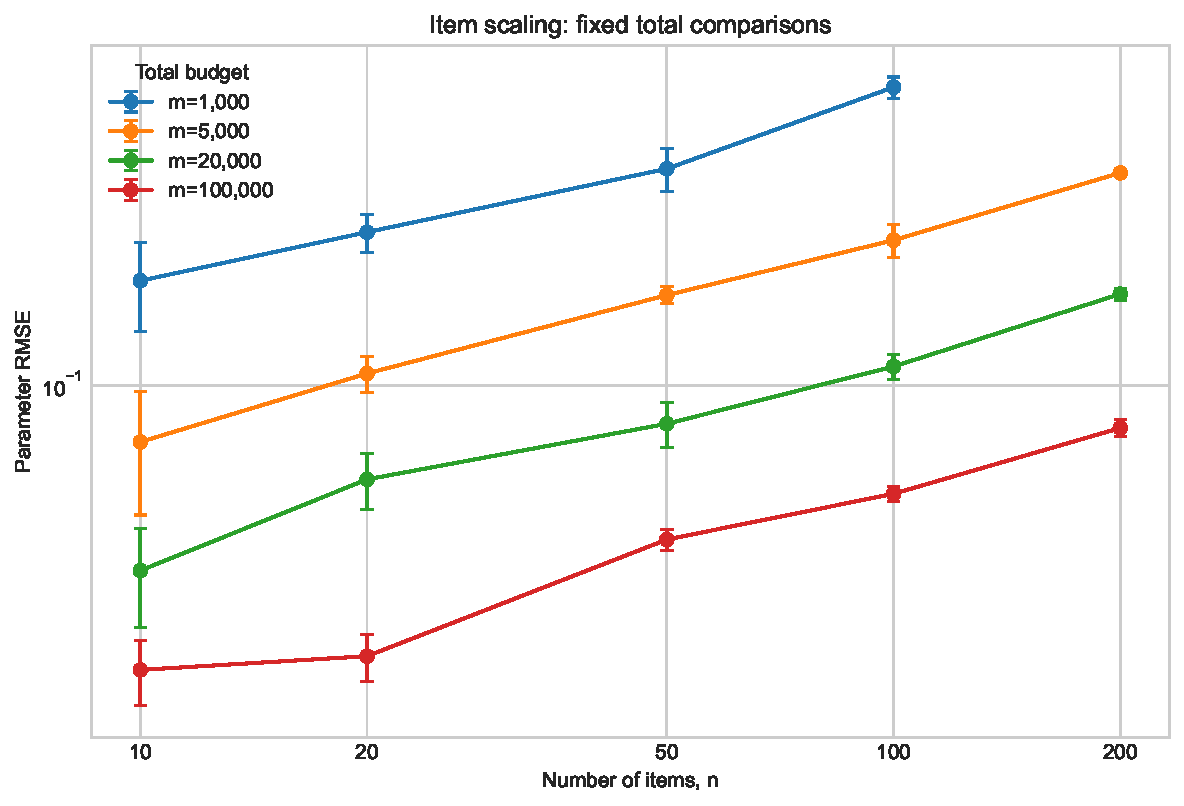
\includegraphics[width=0.82\textwidth]{images/experiments/bradley_terry/bt_choix_recovery_vs_items_fixed_m.pdf}
    \caption{Choix parameter-recovery RMSE versus the number of items at fixed total comparison budgets. Points show means over converged runs, and error bars show one standard deviation.}
    \label{fig:phase1-choix-items-fixed-m}
\end{figure}

\paragraph{Number of Items at Fixed Comparisons per Item}
We also compare settings with $m/n=100$ and $m/n=500$.
Here, the total number of comparisons increases with the number of items,
so the expected appearances per item remain fixed at $200$ and $1000$, respectively.
\begin{figure}[htbp]
    \centering
    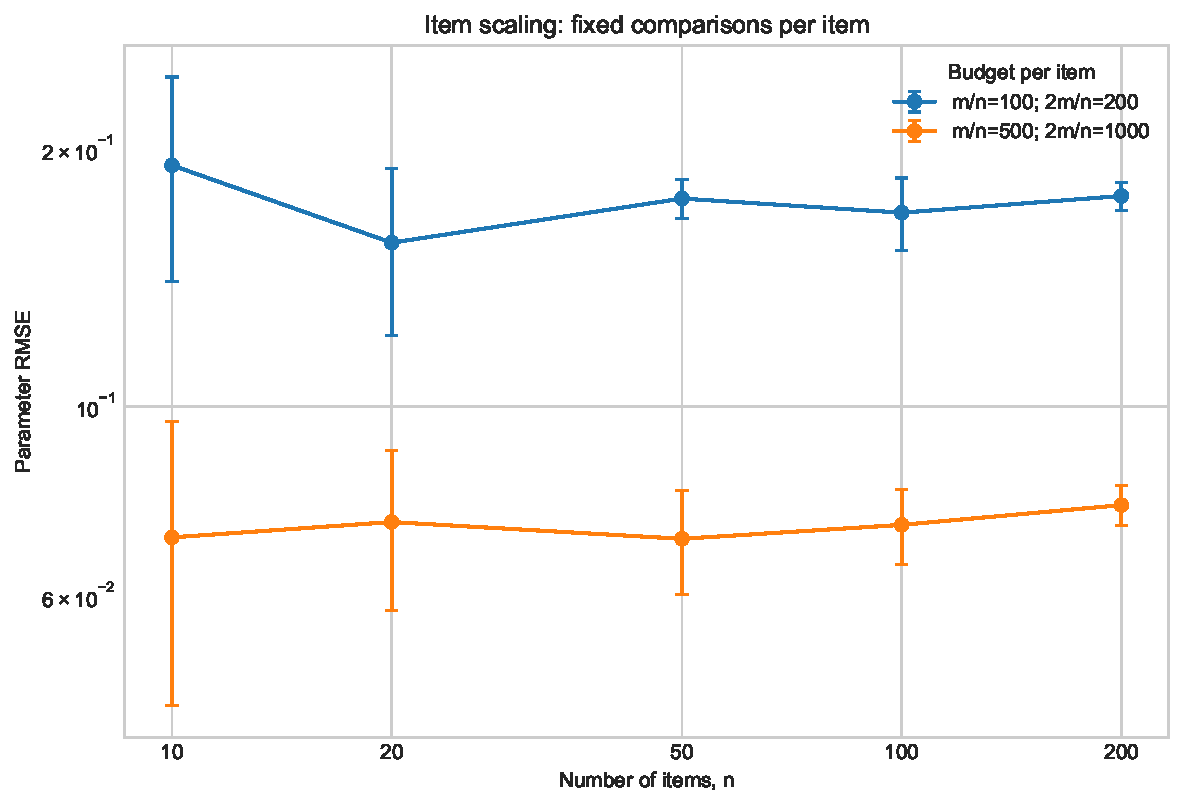
\includegraphics[width=0.82\textwidth]{images/experiments/bradley_terry/bt_choix_recovery_vs_items_fixed_ratio.pdf}
    \caption{Choix parameter-recovery RMSE versus the number of items at fixed $m/n$. Error bars show one standard deviation across converged runs.}
    \label{fig:phase1-choix-items-fixed-ratio}
\end{figure}

Only runs with a finite MLE and a converged fit are included in the recovery summaries.
At $n=200$ and $m=1000$, none of the five runs has a finite MLE, so no RMSE point is shown for that setting.
\FloatBarrier

\subsubsection{Parameter Recovery Using Gradient Descent}
\notebooksource{https://github.com/rbhdsks/Learning-from-Comparison-Data-Master-Thesis-Project-/blob/cc7a5ab5ccf2ef462020f26919576bf275fa4105/notebooks/experiments/Bradley_Terry_Model/From\%20Scratch/01_BradleyTerry_recovery.ipynb}{01_BradleyTerry_recovery.ipynb}

\paragraph{Baseline Parameter Recovery}

The first experiment checks whether the parameters used to generate
simulated Bradley--Terry comparisons can be recovered from the observed
data.

We consider \(n=10\) items. The true parameter vector is constructed
using equally spaced values between \(-1.5\) and \(1.5\). The vector is
centred so that
\begin{equation}
    \sum_{i=1}^{n}\theta_i=0.
\end{equation}

A total of \(m=1000\) pairwise comparisons are generated. Each pair is
sampled uniformly, and the winner is sampled according to the
Bradley--Terry probability in \cref{eq:bradley-terry}. The random seed is
fixed at \(20260831\) to make the experiment reproducible.

The unknown parameters are estimated by minimizing the average negative
log-likelihood using gradient descent. The learning rate is set to
\(0.1\), and the optimizer is run for a maximum of \(1000\) iterations.

The parameter-recovery error is measured using the root mean squared
error
\begin{equation}
    \operatorname{RMSE}
    =
    \sqrt{
        \frac{1}{n}
        \sum_{i=1}^{n}
        \left(
            \widehat{\theta}_i-\theta_i
        \right)^2
    },
    \label{eq:btl-recovery-rmse}
\end{equation}
where \(\theta_i\) is the true parameter and
\(\widehat{\theta}_i\) is its estimate.

\begin{table}[htbp]
    \centering
    \caption{Configuration and result of the baseline
    Bradley--Terry parameter-recovery experiment.}
    \label{tab:btl-baseline-recovery}
    \begin{tabular}{lc}
        \toprule
        Quantity & Value \\
        \midrule
        Number of items, \(n\) & \(10\) \\
        Number of comparisons, \(m\) & \(1000\) \\
        Random seed & \(20260831\) \\
        Learning rate & \(0.1\) \\
        Maximum iterations & \(1000\) \\
        Parameter-recovery RMSE & \(0.1224\) \\
        \bottomrule
    \end{tabular}
\end{table}

\begin{figure}[htbp]
    \centering
    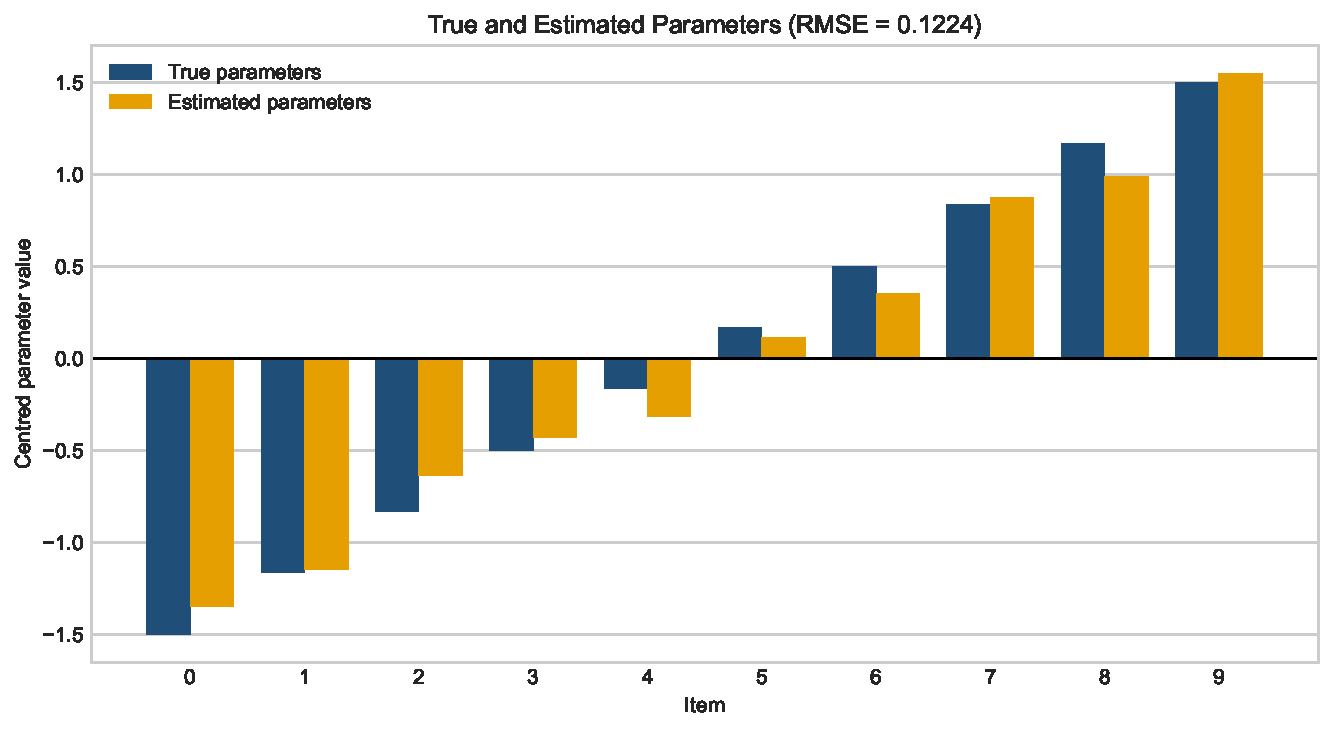
\includegraphics[
        width=0.90\textwidth
    ]{images/experiments/bradley_terry/baseline_parameter_recovery.pdf}
    \caption{Comparison of the true and estimated parameters for the
    baseline Bradley--Terry experiment with \(10\) items and \(1000\)
    pairwise comparisons.}
    \label{fig:btl-baseline-recovery}
\end{figure}

As shown in \cref{fig:btl-baseline-recovery}, the estimated parameters
follow the ordering and approximate magnitudes of the true parameters.
The parameter-recovery RMSE for this simulated dataset is \(0.1224\).

This result provides a baseline example of parameter recovery. Since it
is obtained from a single simulated dataset, it does not describe the
variation across independent datasets. Repeated experiments are used in
the next subsection to study how the recovery error changes with the
number of observed comparisons.

\paragraph{Effect of the Number of Comparisons}

The second experiment studies how the number of observed pairwise
comparisons affects parameter recovery. The number of items is fixed at
\(n=10\), and the same centred true parameter vector used in the
baseline experiment is retained.

The number of comparisons is varied over
\begin{equation}
    m
    \in
    \{50,100,200,500,1000,2000,5000\}.
\end{equation}

For each value of \(m\), the experiment is repeated independently
\(20\) times. A new comparison dataset is generated in every run, while
the true parameters, pair-sampling method, learning rate, and maximum
number of gradient-descent iterations are kept fixed. The mean
parameter-recovery RMSE and its standard deviation are then computed
over the \(20\) runs.

\begin{table}[htbp]
    \centering
    \caption{Parameter-recovery error for different numbers of
    pairwise comparisons. Each result is computed over \(20\)
    independent runs.}
    \label{tab:btl-comparison-scaling}
    \begin{tabular}{rcc}
        \toprule
        Number of comparisons
        & Mean RMSE
        & Standard deviation \\
        \midrule
        \(50\)   & \(0.7225\) & \(0.2172\) \\
        \(100\)  & \(0.4600\) & \(0.1247\) \\
        \(200\)  & \(0.3213\) & \(0.0819\) \\
        \(500\)  & \(0.1786\) & \(0.0487\) \\
        \(1000\) & \(0.1412\) & \(0.0388\) \\
        \(2000\) & \(0.1095\) & \(0.0309\) \\
        \(5000\) & \(0.0780\) & \(0.0203\) \\
        \bottomrule
    \end{tabular}
\end{table}

\begin{figure}[htbp]
    \centering
    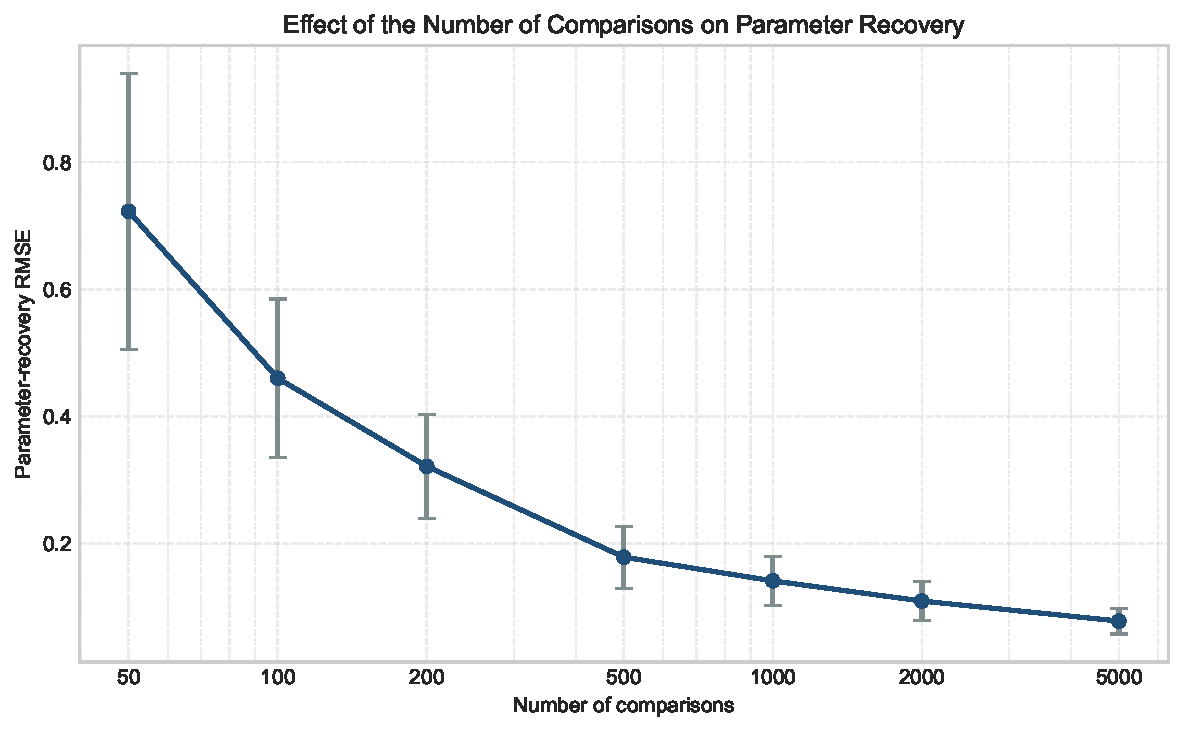
\includegraphics[
        width=0.68\textwidth
    ]{images/experiments/bradley_terry/recovery_error_vs_comparisons.pdf}
    \caption{Mean Bradley--Terry parameter-recovery RMSE as the number
    of comparisons increases. The error bars show one standard
    deviation across \(20\) independent runs.}
    \label{fig:btl-recovery-vs-comparisons}
\end{figure}

As shown in \cref{tab:btl-comparison-scaling,fig:btl-recovery-vs-comparisons},
the mean parameter-recovery RMSE decreases as the number of observed
comparisons increases. It decreases from \(0.7225\) with \(50\)
comparisons to \(0.0780\) with \(5000\) comparisons.

The standard deviation also decreases from \(0.2172\) to \(0.0203\).
Thus, in this experimental setting, increasing the amount of observed
comparison data improves both the average recovery accuracy and the
consistency of the estimates across independent datasets.

\subsubsection{Comparison of Optimization Methods}
\notebooksource{https://github.com/rbhdsks/Learning-from-Comparison-Data-Master-Thesis-Project-/blob/cc7a5ab5ccf2ef462020f26919576bf275fa4105/notebooks/experiments/Bradley_Terry_Model/From\%20Scratch/04_BradleyTerry_MLE_Optimizations.ipynb}{04_BradleyTerry_MLE_Optimizations.ipynb}

\paragraph{Experimental Setup}

The Bradley--Terry negative log-likelihood was minimized using five
optimization methods: full-batch gradient descent, stochastic gradient
descent (SGD), mini-batch gradient descent, gradient descent with
momentum, and Adam.

Each method was implemented in two ways: a handcrafted implementation
and an implementation using PyTorch. The same simulated comparison
dataset and initial parameter vector were used for all methods.

A maximum budget of \(10{,}000\) epochs was used. Convergence was
measured using the norm of the gradient evaluated on the complete
dataset. The convergence tolerance was set to

\begin{equation}
    \left\lVert \nabla \mathcal{L}(\boldsymbol{\theta}) \right\rVert_2
    \leq 10^{-4}.
\end{equation}

For easier comparison, define the convergence ratio

\begin{equation}
    r
    =
    \frac{
        \left\lVert
        \nabla \mathcal{L}(\boldsymbol{\theta})
        \right\rVert_2
    }{
        10^{-4}
    }.
\end{equation}

Thus, a run satisfies the convergence criterion when \(r\leq 1\).

\paragraph{Final Solution Quality}

Table~\ref{tab:optimizer-comparison} summarizes the parameter-recovery
error, convergence ratio, and relative runtime. Here, H and P denote
the handcrafted and PyTorch implementations, respectively.

\begin{table}[H]
    \centering
    \caption{Comparison of the optimization methods. The runtime ratio
    is PyTorch runtime divided by handcrafted runtime.}
    \label{tab:optimizer-comparison}
    \small
    \begin{tabular}{lccc}
        \toprule
        Optimizer
        & RMSE (H/P)
        & \(r\) (H/P)
        & Runtime ratio (P/H) \\
        \midrule
        Full-batch GD
        & \(0.0381/0.0381\)
        & \(1.00/1.00\)
        & \(1.34\) \\

        SGD
        & \(0.0393/0.0395\)
        & \(4.80/4.54\)
        & \(2.59\) \\

        Mini-batch GD
        & \(0.0384/0.0387\)
        & \(0.90/6.31\)
        & \(27.82\) \\

        Momentum GD
        & \(0.0404/0.0360\)
        & \(7.92/9.82\)
        & \(2.15\) \\

        Adam
        & \(0.0408/0.0438\)
        & \(24.94/29.12\)
        & \(2.31\) \\
        \bottomrule
    \end{tabular}
\end{table}

The recovery RMSE values are similar across the different methods,
lying between \(0.0360\) and \(0.0438\). Therefore, all methods produced
parameter estimates close to the true parameters in this experiment.
However, similar recovery errors do not imply that every method
satisfied the numerical convergence criterion.

\paragraph{Convergence Criterion}

Figure~\ref{fig:optimizer-convergence-distance} shows the final
gradient norm relative to the selected tolerance.

\begin{figure}[H]
    \centering
    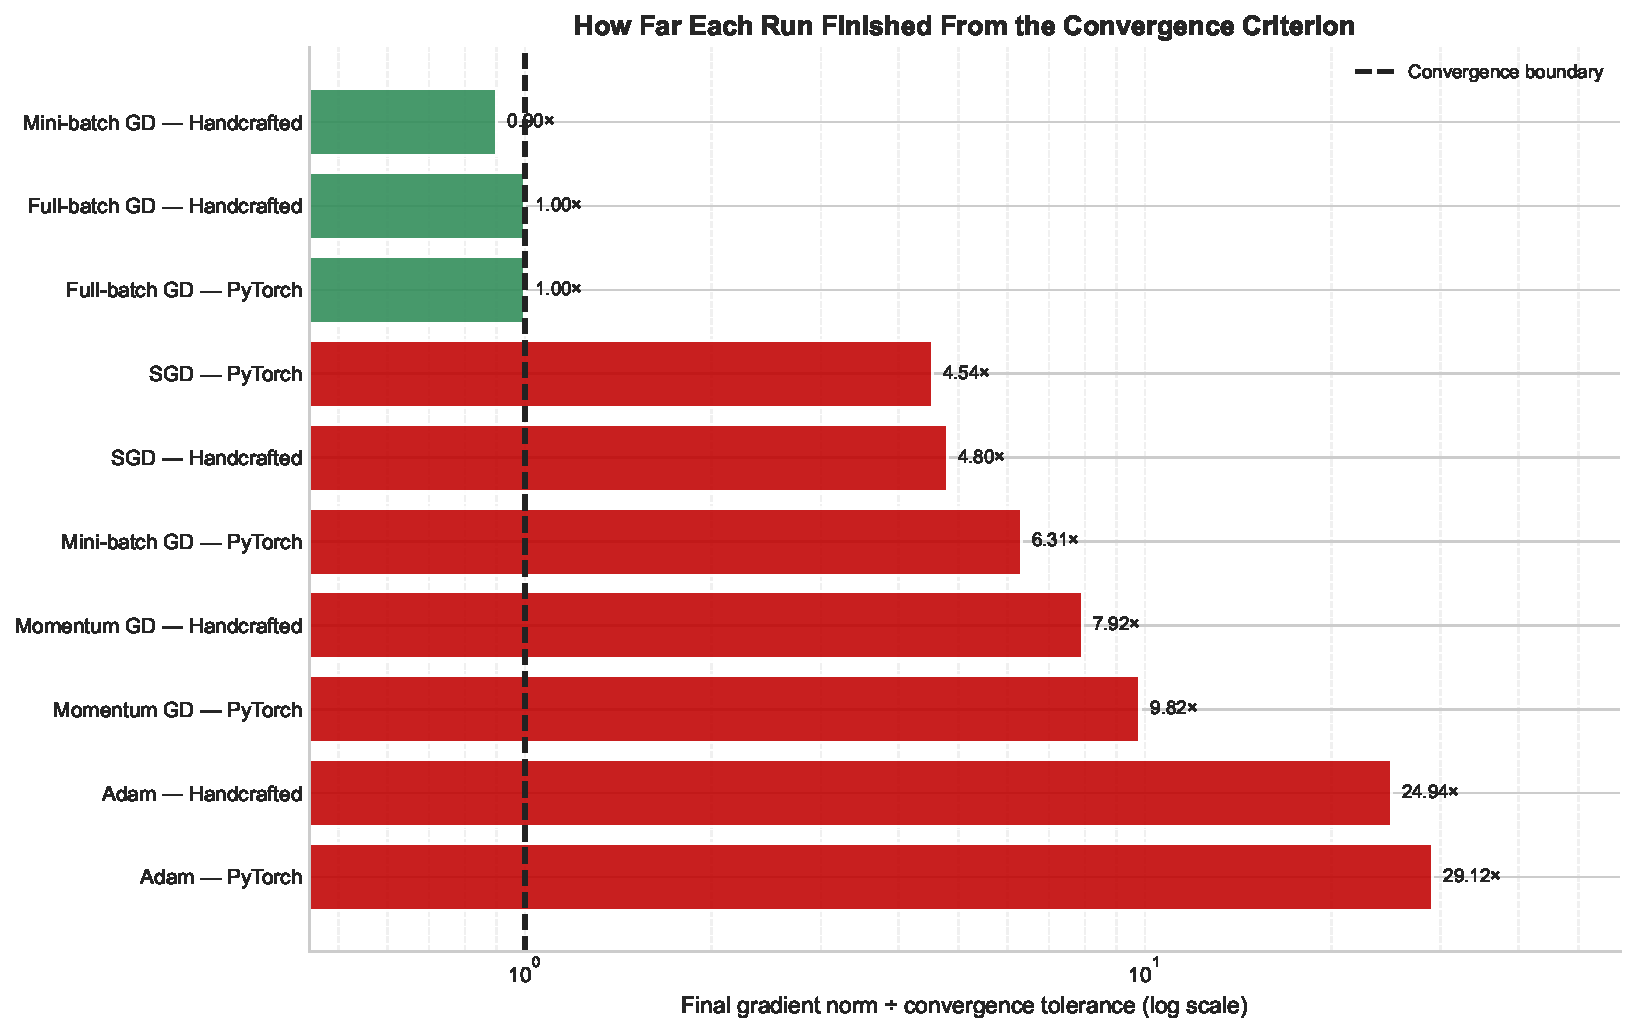
\includegraphics[
        width=0.88\textwidth
    ]{images/experiments/bradley_terry/optimization/fixed_budget/06_distance_from_convergence.pdf}

    \caption{Final gradient norm relative to the convergence tolerance.
    Values at or below one satisfy the convergence criterion.}
    \label{fig:optimizer-convergence-distance}
\end{figure}

Both implementations of full-batch gradient descent satisfied the
convergence criterion. The handcrafted mini-batch implementation also
satisfied the criterion. The remaining methods did not reach the
specified tolerance within the fixed epoch budget.

In particular, stochastic methods continue to fluctuate near a
solution because their updates are computed using individual
observations or mini-batches. Consequently, a small recovery error may
still be obtained even when the full-gradient norm remains above the
strict convergence tolerance.

\paragraph{Handcrafted and PyTorch Runtime}

Figure~\ref{fig:pytorch-runtime-overhead} compares the runtime of the
PyTorch implementation with its corresponding handcrafted
implementation.

\begin{figure}[H]
    \centering
    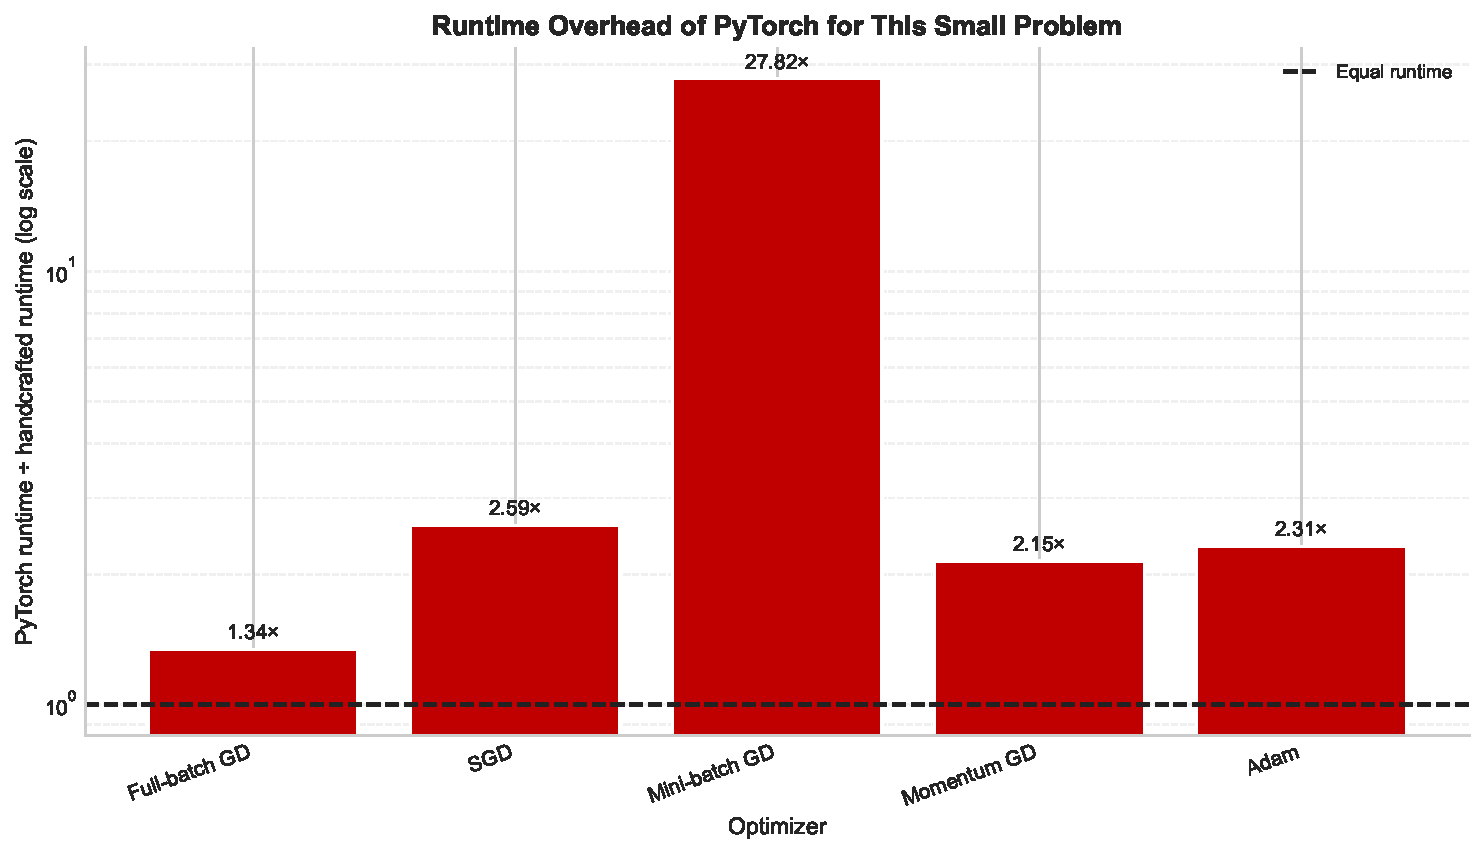
\includegraphics[
        width=0.82\textwidth
    ]{images/experiments/bradley_terry/optimization/fixed_budget/07_pytorch_to_handcrafted_runtime_ratio.pdf}

    \caption{Ratio of PyTorch runtime to handcrafted runtime for each
    optimization method. A value greater than one indicates that the
    PyTorch implementation required more time.}
    \label{fig:pytorch-runtime-overhead}
\end{figure}

For this Bradley--Terry problem, the handcrafted implementations
were faster than their PyTorch counterparts, and among all those Adam optimizer performed well. The additional runtime
is consistent with the overhead introduced by tensor operations and
automatic differentiation on a small CPU-based problem.

This observation is specific to the present implementation and problem
size. It should not be interpreted as a general comparison of PyTorch
and handcrafted optimization, since PyTorch may become advantageous
for larger models, larger datasets, or GPU-based computation.

% =========================================================
% CHAPTER 3
% =========================================================
% =========================================================
% CHAPTER 3
% Cleaned version through the full-rank CDM reparameterisation
% =========================================================


\FloatBarrier
\subsection{Computational Scaling of the Full and Low-Rank CDM}
\notebooksource{https://github.com/rbhdsks/Learning-from-Comparison-Data-Master-Thesis-Project-/blob/cc7a5ab5ccf2ef462020f26919576bf275fa4105/notebooks/experiments/Context_Dependent_Model/Low\%20Rank\%20CDM/01-FullvsLowrankResourceScaling.ipynb}{01-FullvsLowrankResourceScaling.ipynb}
\label{sec:full-low-rank-resource-scaling}

The low-rank model uses fewer trainable parameters than the full CDM.
We now examine how this reduction affects the resources required for
model fitting as the number of items increases. The experiment compares
training time, average time per update, parameter storage, and process
memory. It uses the existing dense-matrix implementations of the models.

\subsubsection{Experimental Setup}

The number of items was varied over
$n\in\{250,500,1000,2000,3000,5000\}$. For each item count, we generated
1,000 observations from a full CDM with parameter scale $0.4$ and
choice-set sizes two and three. The full model and low-rank models with
$r\in\{1,2,3\}$ were fitted to the same observations within each repeat.
Five repeats were performed for every setting, giving 120 successful
model fits in total. Dataset fingerprints were checked to verify that
the four models received the same observations within each repeat.

All models were fitted using Adam with learning rate $0.05$ for exactly
1,000 updates. Computation was performed on the CPU using
\texttt{float64} and one PyTorch computational thread. The base random
seed was 20260831. Each fit ran in a separate process, and the order of
the fits was randomly shuffled.

The training time includes the optimization loop. Data generation, model
construction, and the final loss and gradient evaluation are outside
this timing interval. Since the update budget is fixed, this experiment
measures computational cost rather than time to convergence. It also
does not compare parameter recovery or held-out predictive performance.

\subsubsection{Number of Trainable Parameters and Parameter Storage}

The full implementation stores an $n\times n$ trainable matrix. The
low-rank implementation stores two $n\times r$ factor matrices. Thus,
the numbers of trainable entries are
\begin{equation}
    N_{\mathrm{full}}=n^2,
    \qquad
    N_{\mathrm{low\text{-}rank}}=2nr.
    \label{eq:resource-trainable-entries}
\end{equation}
These counts describe the entries stored by the implementation. They
are not the numbers of identifiable free parameters discussed earlier.
For a fixed rank, the number of trainable entries grows linearly with
$n$, whereas the full matrix requires quadratic storage.

For example, at $n=5000$, the full model contains 25,000,000 trainable
entries. The rank-one, rank-two, and rank-three models contain 10,000,
20,000, and 30,000 entries, respectively. The rank-one model therefore
uses 2,500 times fewer trainable entries than the full model.

Each \texttt{float64} entry occupies eight bytes. The storage of the
trainable tensors, measured in MiB, is therefore
\begin{equation}
    S_{\mathrm{parameters}}
    =\frac{8N_{\mathrm{parameters}}}{2^{20}}.
    \label{eq:resource-parameter-storage}
\end{equation}
This quantity excludes gradients, optimizer states, observations, and
temporary allocations. It should therefore be distinguished from the
total memory occupied by the process.

\begin{figure}[htbp]
    \centering
    \begin{subfigure}{0.80\textwidth}
        \centering
        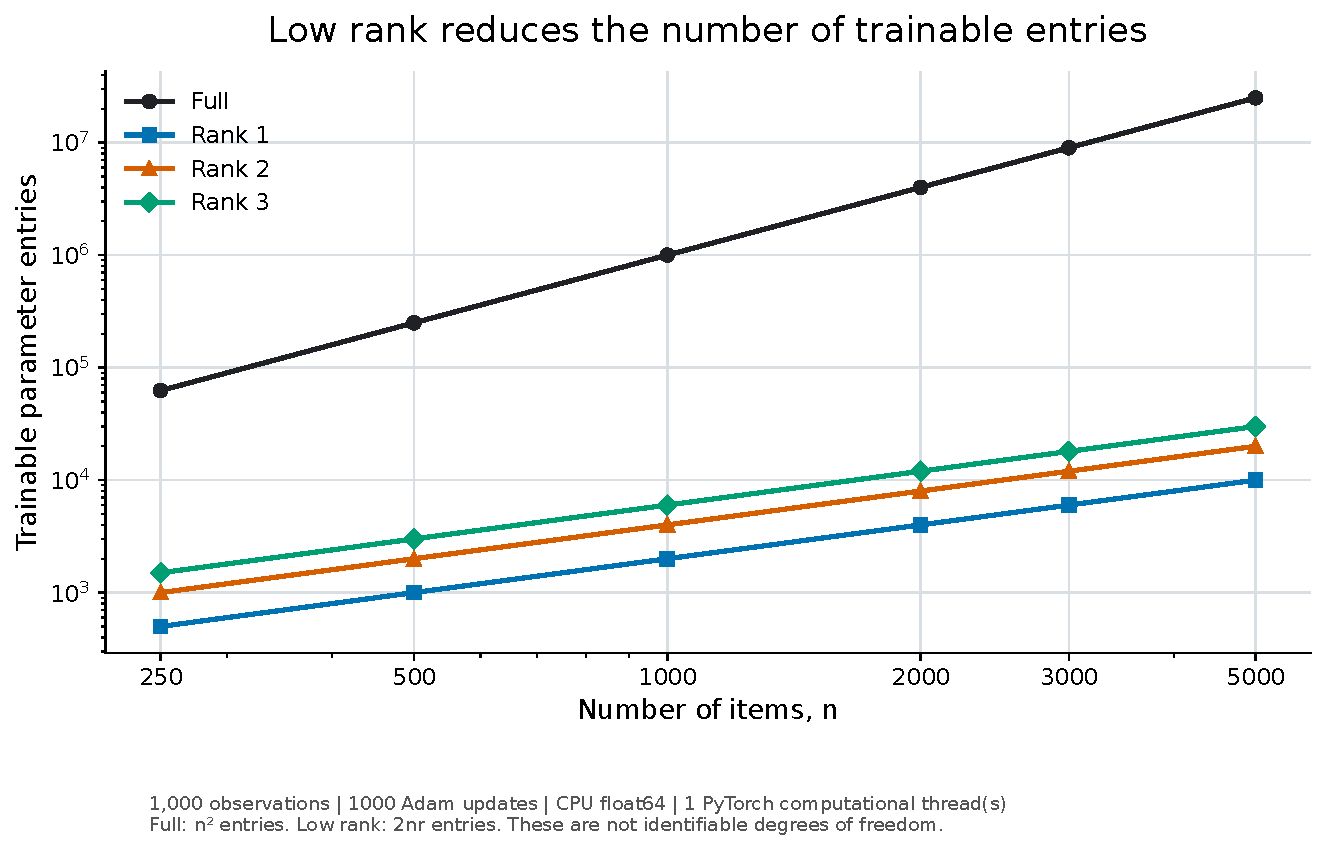
\includegraphics[width=\linewidth]{images/experiments/context_dependent_model/05_full_vs_low_rank_resource_scaling/20261021T202900_245293Z/01_parameter_count.pdf}
        \caption{Number of trainable entries.}
    \end{subfigure}
    \par\medskip
    \begin{subfigure}{0.80\textwidth}
        \centering
        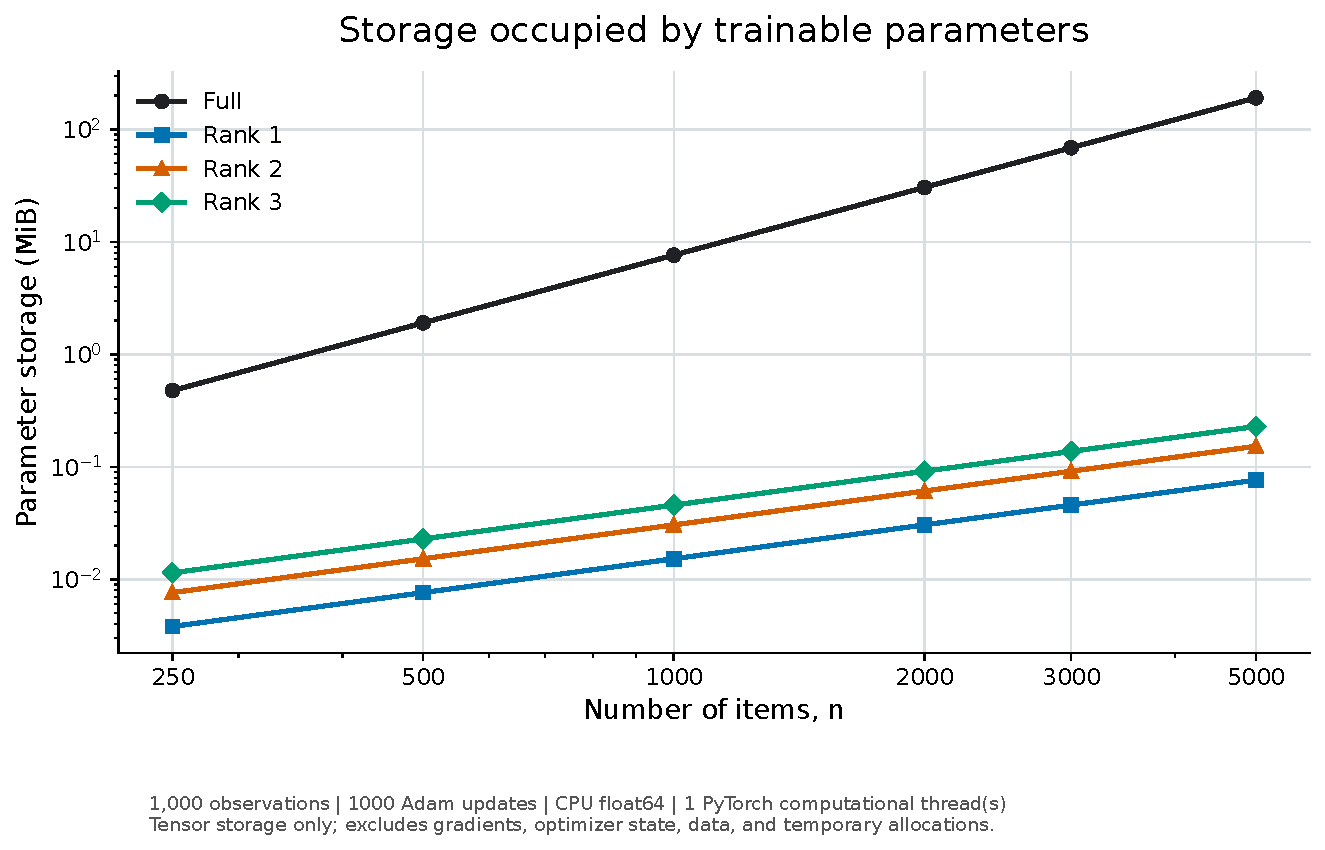
\includegraphics[width=\linewidth]{images/experiments/context_dependent_model/05_full_vs_low_rank_resource_scaling/20261021T202900_245293Z/02_parameter_storage.pdf}
        \caption{Storage occupied by trainable tensors.}
    \end{subfigure}
    \caption{Trainable entries and their tensor storage for the full and low-rank CDM. Storage excludes gradients, optimizer states, data, and temporary allocations.}
    \label{fig:resource-parameters}
\end{figure}

\subsubsection{Training Time and Average Time per Update}

Table~\ref{tab:resource-scaling-summary} reports the mean training time,
its standard deviation, and the mean sampled peak process memory across
the five repeats. Training time increased substantially with the number
of items for all four models.

\begin{table}[htbp]
    \centering
    \caption{Computational resources for the full and low-rank CDM.
    Time is measured over 1,000 Adam updates. Each setting has five
    repeats. Peak RSS is the mean sampled peak process memory.}
    \label{tab:resource-scaling-summary}
    \begingroup
    \singlespacing
    \small
    \resizebox{\textwidth}{!}{%
        \begin{tabular}{lrrrrrr}
\toprule
Model & Items & Runs & Parameters & Time mean (s) & Time SD (s) & Peak RSS (MiB) \\
\midrule
Full & 250 & 5 & 62500 & 0.876 & 0.022 & 299.559 \\
Full & 500 & 5 & 250000 & 2.770 & 0.046 & 320.503 \\
Full & 1000 & 5 & 1000000 & 14.643 & 0.320 & 357.125 \\
Full & 2000 & 5 & 4000000 & 60.975 & 1.281 & 470.828 \\
Full & 3000 & 5 & 9000000 & 137.423 & 1.017 & 674.728 \\
Full & 5000 & 5 & 25000000 & 413.346 & 2.486 & 1249.312 \\
Rank 1 & 250 & 5 & 500 & 0.829 & 0.020 & 312.606 \\
Rank 1 & 500 & 5 & 1000 & 2.306 & 0.105 & 316.431 \\
Rank 1 & 1000 & 5 & 2000 & 12.089 & 0.337 & 320.850 \\
Rank 1 & 2000 & 5 & 4000 & 49.681 & 1.108 & 395.331 \\
Rank 1 & 3000 & 5 & 6000 & 110.941 & 2.039 & 530.866 \\
Rank 1 & 5000 & 5 & 10000 & 307.714 & 4.728 & 1023.025 \\
Rank 2 & 250 & 5 & 1000 & 0.822 & 0.025 & 301.675 \\
Rank 2 & 500 & 5 & 2000 & 2.186 & 0.101 & 309.366 \\
Rank 2 & 1000 & 5 & 4000 & 12.400 & 0.137 & 343.231 \\
Rank 2 & 2000 & 5 & 8000 & 51.217 & 0.622 & 418.922 \\
Rank 2 & 3000 & 5 & 12000 & 113.587 & 3.033 & 528.475 \\
Rank 2 & 5000 & 5 & 20000 & 322.378 & 4.124 & 1013.959 \\
Rank 3 & 250 & 5 & 1500 & 0.822 & 0.010 & 287.931 \\
Rank 3 & 500 & 5 & 3000 & 2.145 & 0.112 & 312.275 \\
Rank 3 & 1000 & 5 & 6000 & 12.211 & 0.328 & 339.137 \\
Rank 3 & 2000 & 5 & 12000 & 51.435 & 0.288 & 422.572 \\
Rank 3 & 3000 & 5 & 18000 & 116.987 & 4.034 & 542.128 \\
Rank 3 & 5000 & 5 & 30000 & 319.222 & 7.053 & 1018.731 \\
\bottomrule
\end{tabular}
%
    }
    \endgroup
\end{table}

At $n=5000$, the full model required $413.346\pm2.486$ seconds.
The rank-one, rank-two, and rank-three models required
$307.714\pm4.728$, $322.378\pm4.124$, and $319.222\pm7.053$ seconds,
respectively. Here, the values after $\pm$ are standard deviations across
the five repeats. The low-rank models were approximately 22--26\%
faster at this item count. This reduction is much smaller than the
reduction in the number of trainable entries.

The average time per update was calculated by dividing the training-loop
time by 1,000. It follows the same scaling pattern as total training
time because every model uses the same update budget. Its error bars
describe variation across repeats, rather than variation between
individual updates within a fit.

\begin{figure}[htbp]
    \centering
    \begin{subfigure}{0.80\textwidth}
        \centering
        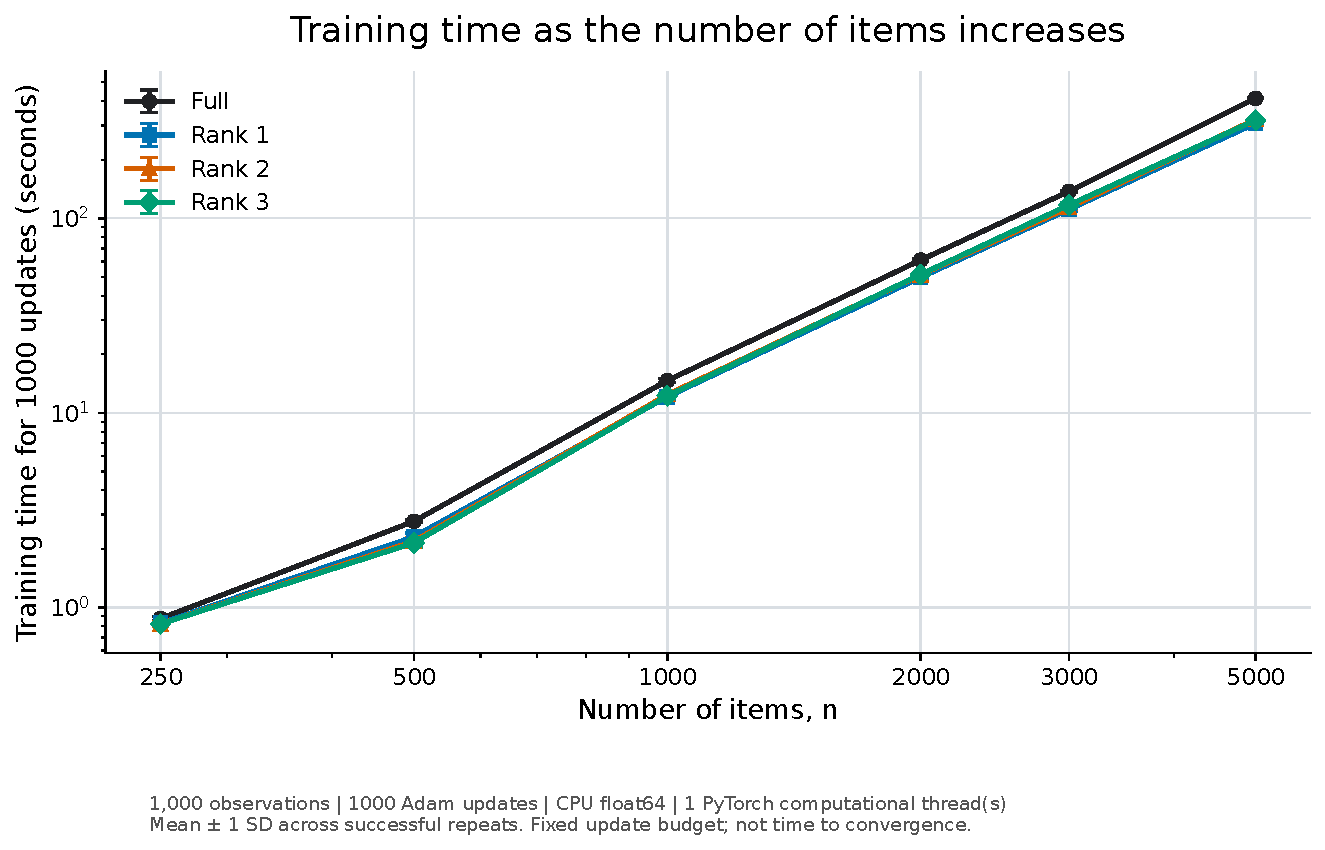
\includegraphics[width=\linewidth]{images/experiments/context_dependent_model/05_full_vs_low_rank_resource_scaling/20261021T202900_245293Z/03_training_time.pdf}
        \caption{Total training-loop time.}
    \end{subfigure}
    \par\medskip
    \begin{subfigure}{0.80\textwidth}
        \centering
        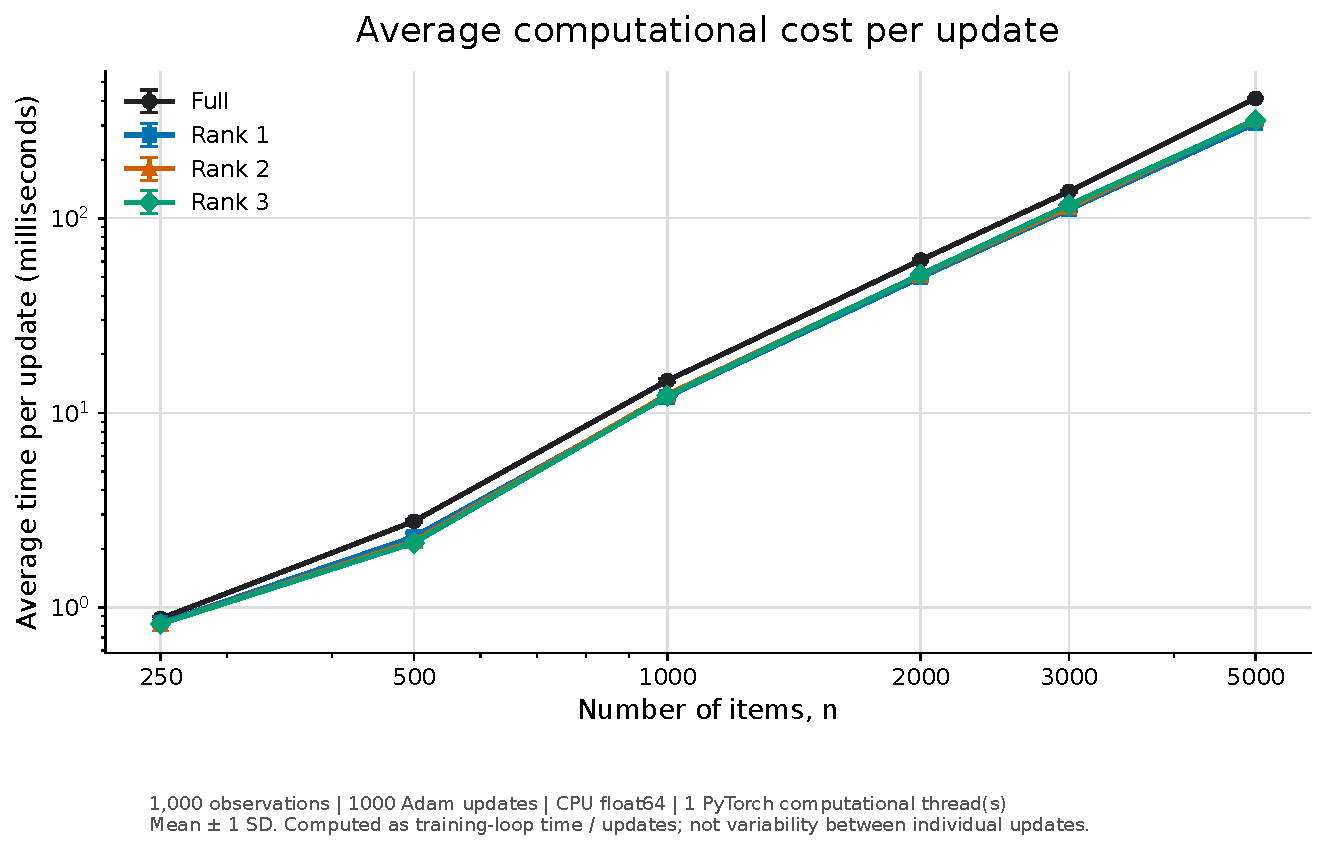
\includegraphics[width=\linewidth]{images/experiments/context_dependent_model/05_full_vs_low_rank_resource_scaling/20261021T202900_245293Z/04_time_per_update.pdf}
        \caption{Average time per update.}
    \end{subfigure}
    \caption{Computational cost as the number of items increases. Points show means across five repeats, and error bars show one standard deviation. Each fit uses 1,000 Adam updates.}
    \label{fig:resource-training-time}
\end{figure}

\subsubsection{Empirical Growth of Training Time}

To describe the observed runtime growth, we fitted a power law to the
mean training times:
\begin{equation}
    t(n)\approx a n^{\alpha},
    \qquad
    \log t(n)\approx\log a+\alpha\log n.
    \label{eq:resource-runtime-power-law}
\end{equation}
The intercept and exponent were estimated by ordinary least squares in
log-log coordinates. Only the four item counts with $n\geq1000$ were
used, and each included setting had all five repeats completed.

\begin{table}[htbp]
    \centering
    \caption{Empirical power-law fits to mean training time for
    $n\in\{1000,2000,3000,5000\}$. The doubling multiplier is
    $2^{\alpha}$. Fit statistics are reported at the precision saved
    by the notebook.}
    \label{tab:resource-runtime-power-law}
    \begingroup
    \singlespacing
    \small
    \resizebox{\textwidth}{!}{%
        \begin{tabular}{lrrrr}
\toprule
Model & Exponent alpha & Log-log R squared & Time multiplier when n doubles & Item counts fitted \\
\midrule
Full & 2.069 & 1.000 & 4.197 & 4 \\
Rank 1 & 2.010 & 1.000 & 4.029 & 4 \\
Rank 2 & 2.021 & 1.000 & 4.059 & 4 \\
Rank 3 & 2.030 & 1.000 & 4.083 & 4 \\
\bottomrule
\end{tabular}
%
    }
    \endgroup
\end{table}

The estimated exponents were $2.069$ for the full model and $2.010$,
$2.021$, and $2.030$ for ranks one, two, and three, respectively.
Thus, the measured training time grew approximately quadratically over
the fitted range for all four models. Under these fitted relationships,
doubling the number of items multiplies the training time by approximately
$4.197$, $4.029$, $4.059$, and $4.083$, respectively.

These exponents describe the observed implementation and item range.
They do not prove an asymptotic complexity bound. In particular, the
linear growth of the number of low-rank trainable entries does not imply
linear training time for the dense implementation used here.

\begin{figure}[htbp]
    \centering
    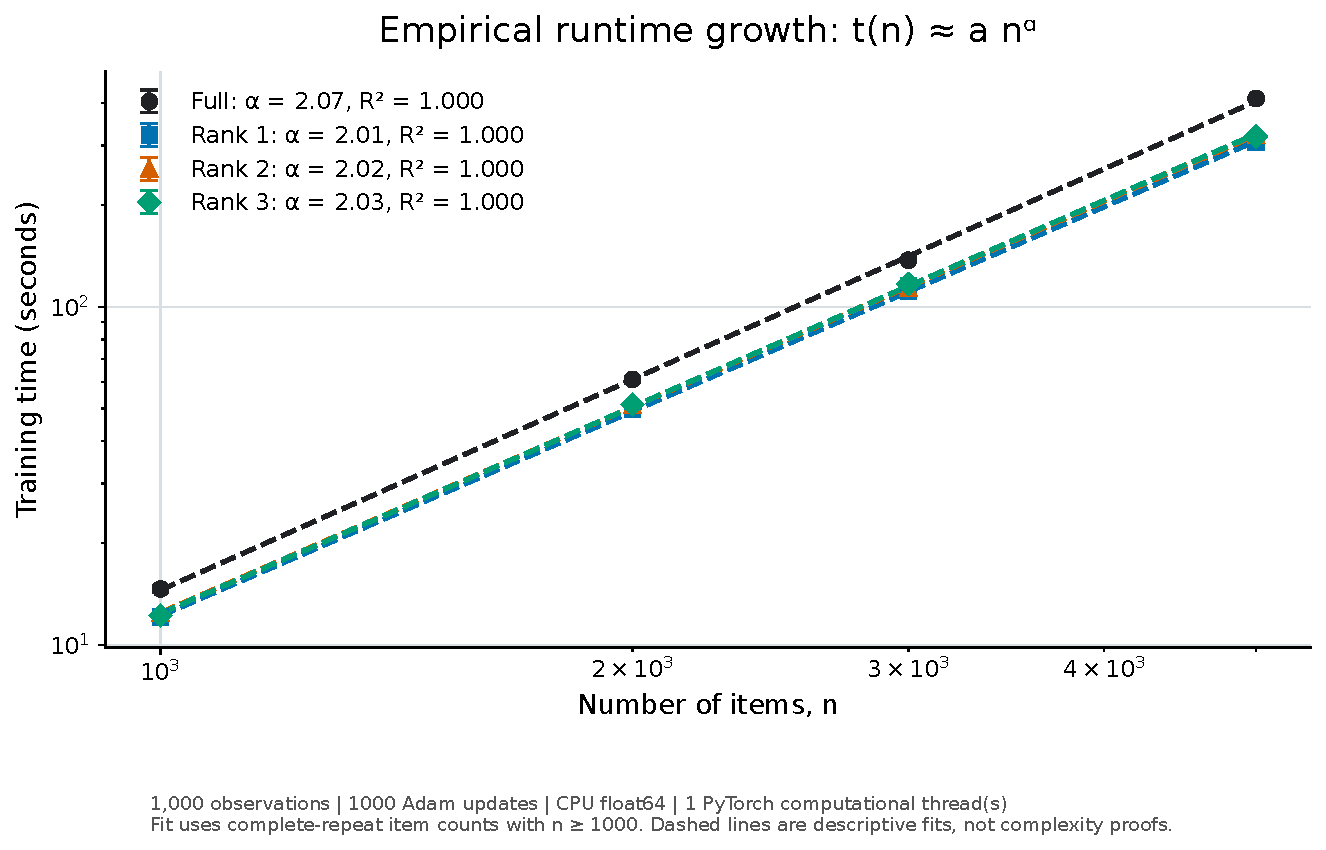
\includegraphics[width=\textwidth]{images/experiments/context_dependent_model/05_full_vs_low_rank_resource_scaling/20261021T202900_245293Z/07_empirical_runtime_exponents.pdf}
    \caption{Empirical power-law fits to training time for $n\geq1000$.
    Points and error bars show the mean and standard deviation across
    five repeats. Dashed lines describe the fitted range and are not
    proofs of asymptotic complexity.}
    \label{fig:resource-runtime-exponents}
\end{figure}

\subsubsection{Process Memory}

Process memory was measured using resident set size (RSS), sampled at
intervals of $0.005$ seconds. The baseline was recorded after data
generation and before model construction. Sampling continued through
model fitting and the final loss and gradient evaluation. The sampled
peak therefore includes the Python/PyTorch process, observations, model
parameters, and allocations made during fitting. It is not a measurement
of parameter storage alone.

At $n=5000$, the mean sampled peak RSS was $1249.312$ MiB for the full
model. The corresponding values were $1023.025$, $1013.959$, and
$1018.731$ MiB for ranks one, two, and three, respectively. Low-rank
parameterization reduced the measured peak at this item count, but the
reduction was much smaller than the parameter-storage reduction.
At the smaller item counts, process overhead and variation between runs
also affect the ordering of the measured peaks.

The notebook additionally records the increase above the baseline:
\begin{equation}
    \Delta\mathrm{RSS}
    =\mathrm{RSS}_{\mathrm{sampled\ peak}}
     -\mathrm{RSS}_{\mathrm{baseline}}.
    \label{eq:resource-rss-increase}
\end{equation}
Both memory measurements are approximate. Periodic sampling can miss
short-lived peaks, and memory retained or reused by the allocator can
affect the increase above the baseline.

\begin{figure}[htbp]
    \centering
    \begin{subfigure}{0.80\textwidth}
        \centering
        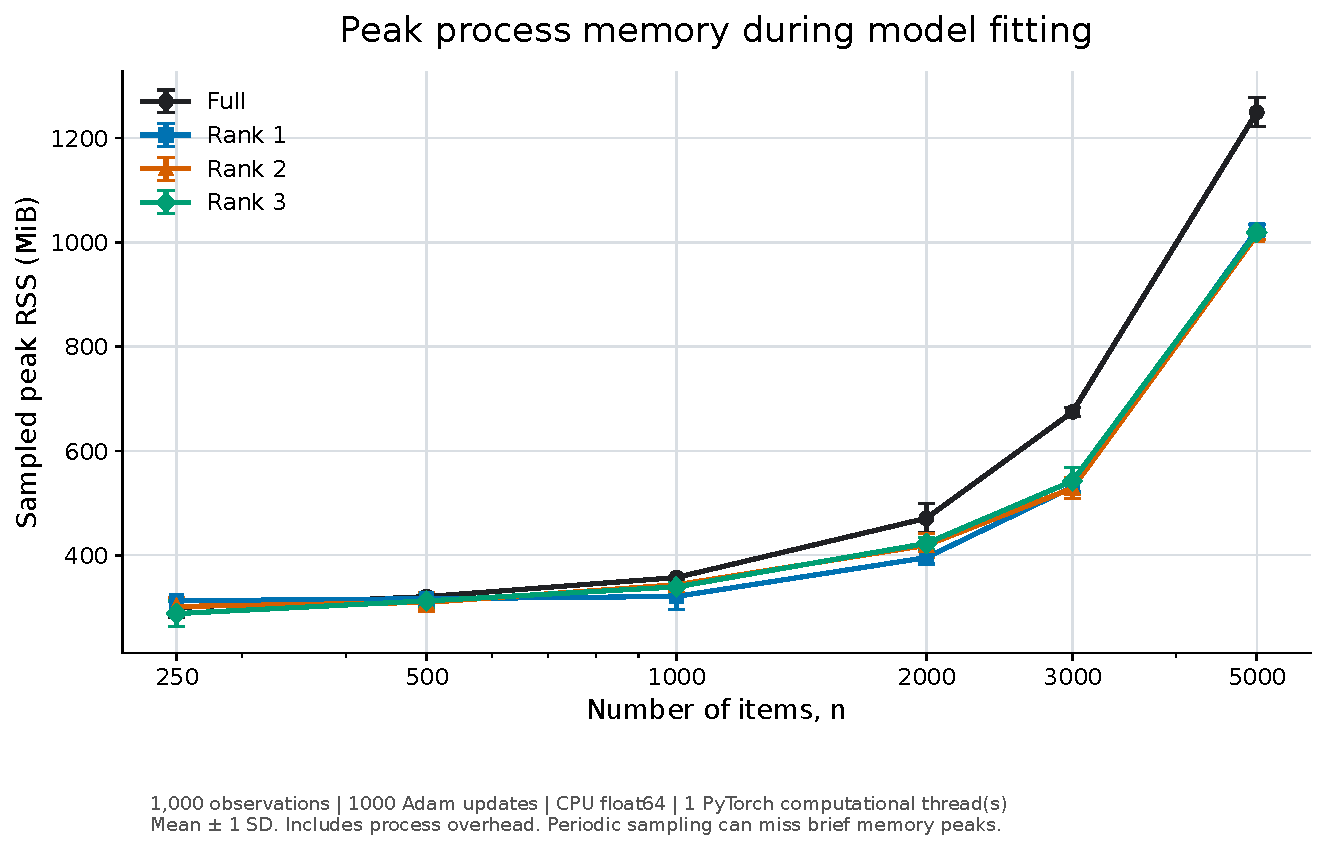
\includegraphics[width=\linewidth]{images/experiments/context_dependent_model/05_full_vs_low_rank_resource_scaling/20261021T202900_245293Z/05_peak_process_memory.pdf}
        \caption{Sampled peak RSS.}
    \end{subfigure}
    \par\medskip
    \begin{subfigure}{0.80\textwidth}
        \centering
        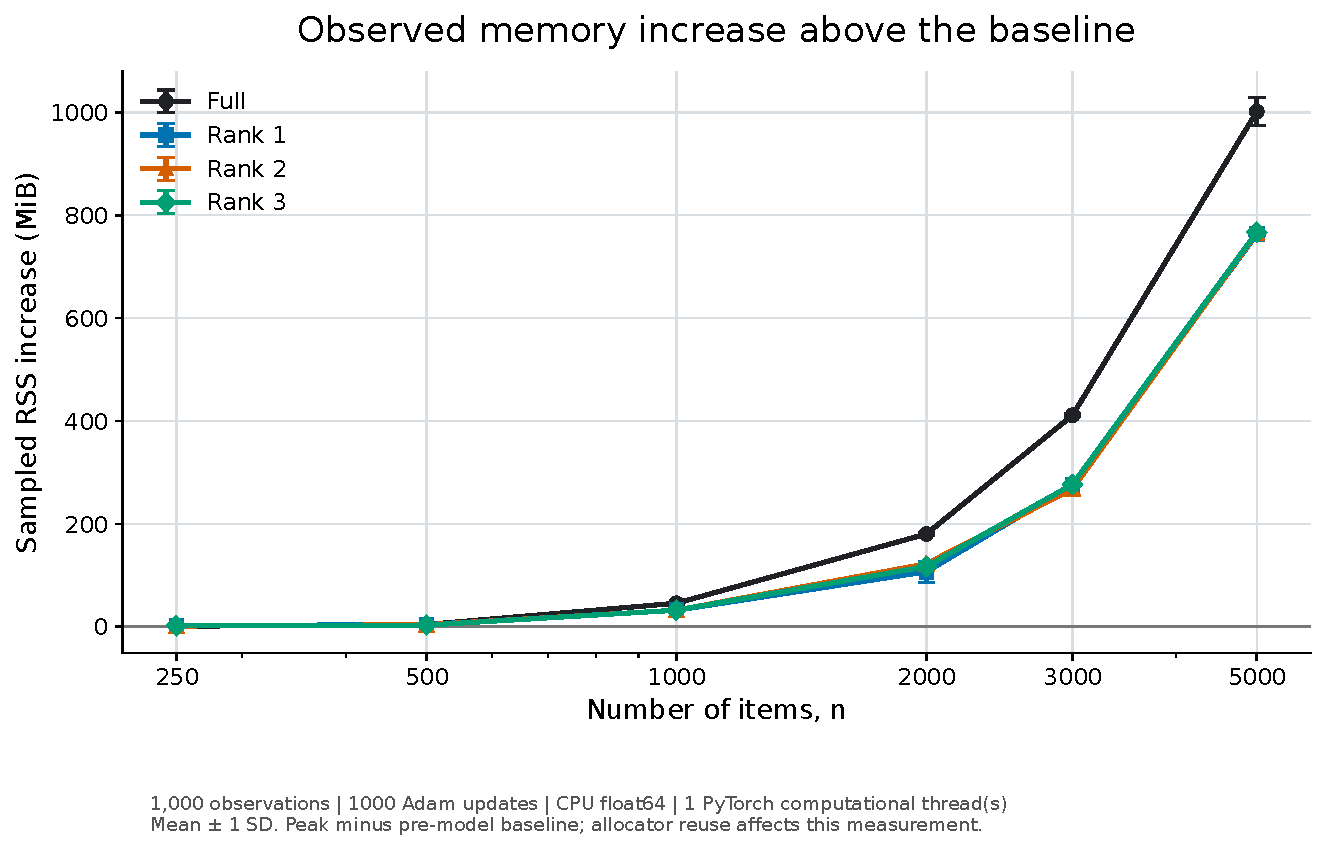
\includegraphics[width=\linewidth]{images/experiments/context_dependent_model/05_full_vs_low_rank_resource_scaling/20261021T202900_245293Z/06_memory_increase.pdf}
        \caption{Sampled peak RSS minus the pre-model baseline.}
    \end{subfigure}
    \caption{Sampled process memory during fitting. Points show means across five repeats, and error bars show one standard deviation. RSS includes process overhead, and periodic sampling can miss brief peaks.}
    \label{fig:resource-process-memory}
\end{figure}

\subsubsection{Summary of scaling experiments.}

So, these experiments show that low-rank parameterization is substantially
reducing the number of trainable parameters. However, parameter count,
training time, and total process memory do not decrease by the same
factor. In these present implementations, the low-rank models still
show approximately quadratic runtime growth over the measured range.
The results therefore separate the storage benefit of the parameterization
from the computational behaviour of the implementation. 



\section{CDM Paper Reproduction}
\null\par
\label{sec:reproduction}
% Fill this only with work you completed and can explain.
% Source material: CDM_Paper_Reproduction notebooks and saved outputs.
% State which paper experiment is being reproduced, what matches/differs,
% completed settings, and limitations. Cite the paper.
% If excluded, redistribute this page to the experiments above.

\section{Discussion and Further Work}
\null\par
\label{sec:discussion}
% Write your own conclusions, tied to specific results in this report.
% Separate completed results from planned work (including cycle detection).
% State limitations and the next steps; do not introduce new results here.

\FloatBarrier
% References share the 15-page limit. Uncomment after adding citations.
% Existing bibliography files can be used without duplicating their entries.
\bibliographystyle{plainnat}
\bibliography{references}

\end{document}
